\chapter{Results}
\label{ch:results}

The results of the experiments conducted in this study are presented in this chapter. The findings are organised according to the research questions outlined in Chapter \ref{ch:intro}. Each section provides a detailed analysis of the results, including relevant figures and tables to support the findings. Detailed analysis of the results will follow in Chapter \ref{ch:discuss}.

\section{General characteristics of storms from the database}

Before modelling, a limited exploratory data analysis was conducted to understand the general characteristics of the filtered dataset assembled for the study. Special attention was paid to the geographic and temporal distribution of the storms. Figure \ref{fig:orography_storm_init_end_kde} shows the density of storm start and end locations within the study region. The distribution is highly concentrated around the Ethiopian Highlands and diminishes quickly closer to the coastline with the Indian Ocean. For the modelling problem, this spatial distribution suggests a strong orographic influence on storm genesis and dissipation.

\begin{figure}[ht]
    \centering
    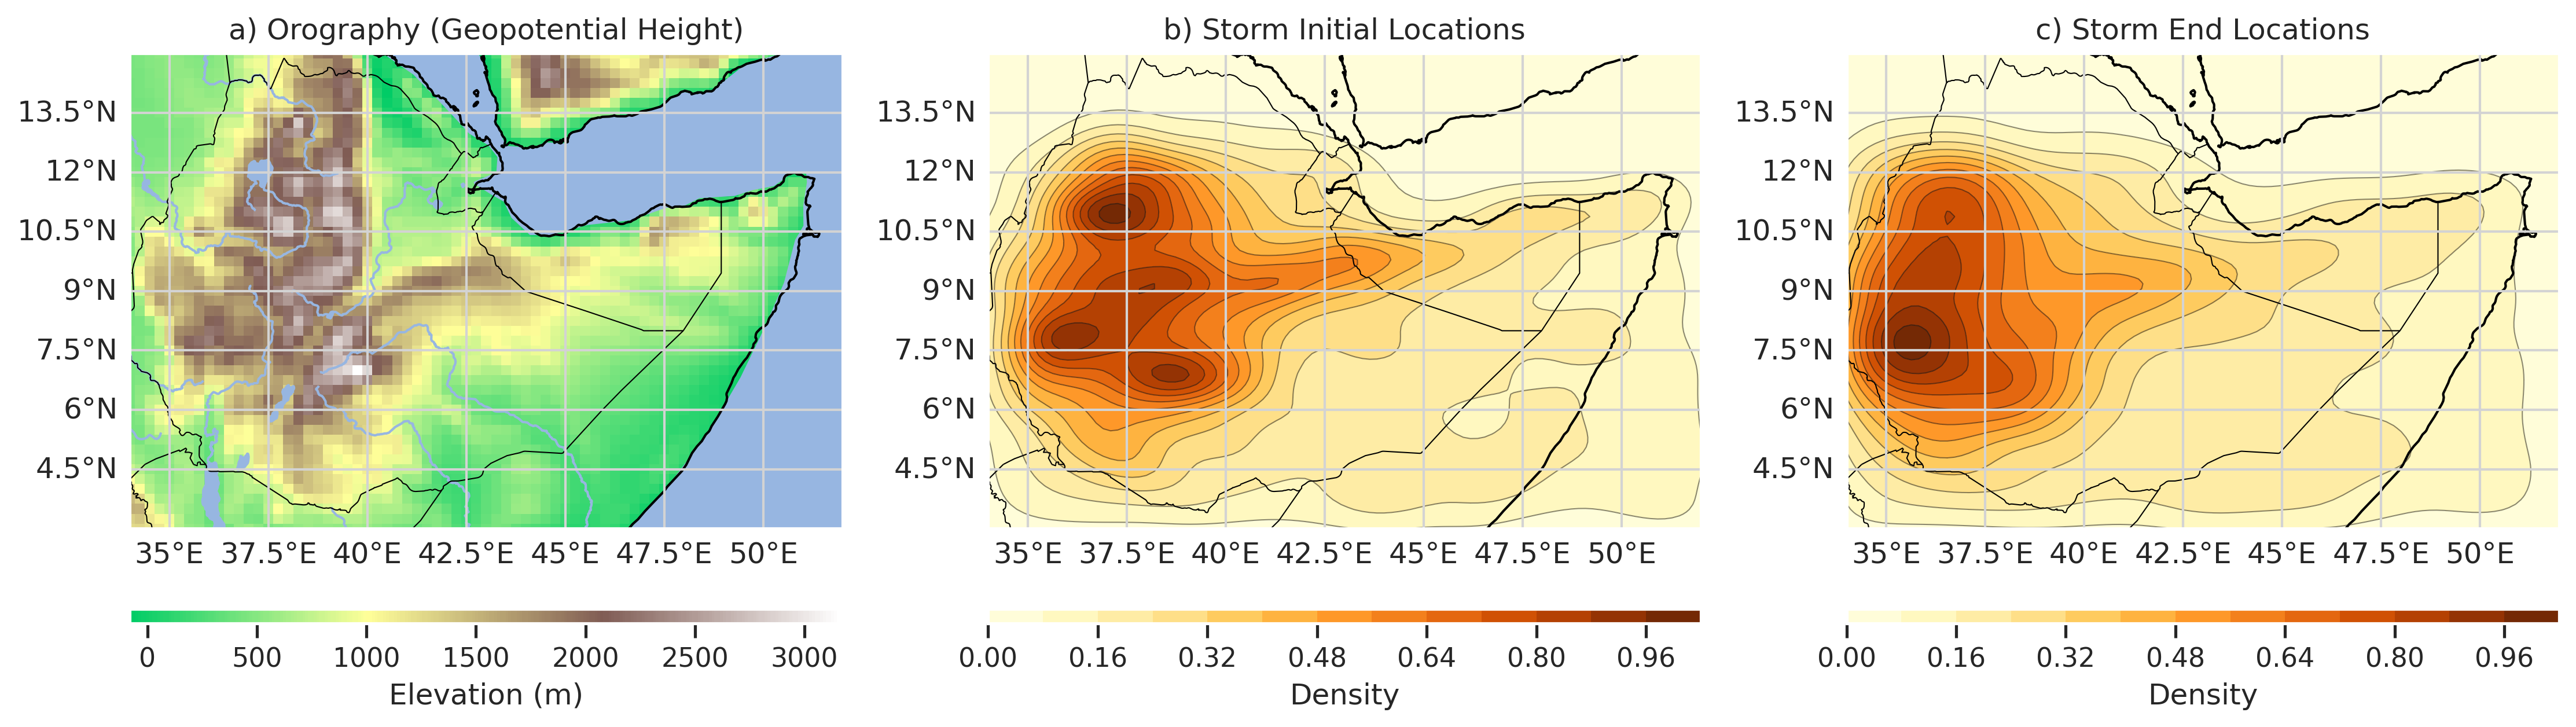
\includegraphics[width=\textwidth]{../figures/generated/exploration/orography_storm_init_end_kde.png}
    \caption{Storm start and end location density. Storms were selected if 1) they last longer than 3 hours to precipitation contributions, and 2) their centroids are located within \degN{3} - \degN{15} and \degE{34} - \degE{52} \citep{Hill2023}. See Chapter \ref{ch:method} for details. Elevation was calculated from \acrshort{era5} geopotential height data.}
    \label{fig:orography_storm_init_end_kde}
\end{figure}

Figure \ref{fig:orography_storm_init_eat_hours_mode_mean} shows the distribution of storm genesis local time with multiple distinct phenomena present. First, although the density of storms of the coast of Somalia is limited, it is clear that storms which form over the ocean tend to form in the early morning hours whereas storms which form over land tend to form in the late afternoon. However, orography also appears to play a role pushing genesis later into the night, with clear anomalies nearly the strong ridge line at \degE{40} in northeast Ethiopia and around the Abaya Lake valley region. This is potentially due to the influence of mountain-valley breezes which can enhance convection in the late evening and early night hours \citep{ZardiDinoandWhiteman2013}.

\begin{figure}[ht]
    \centering
    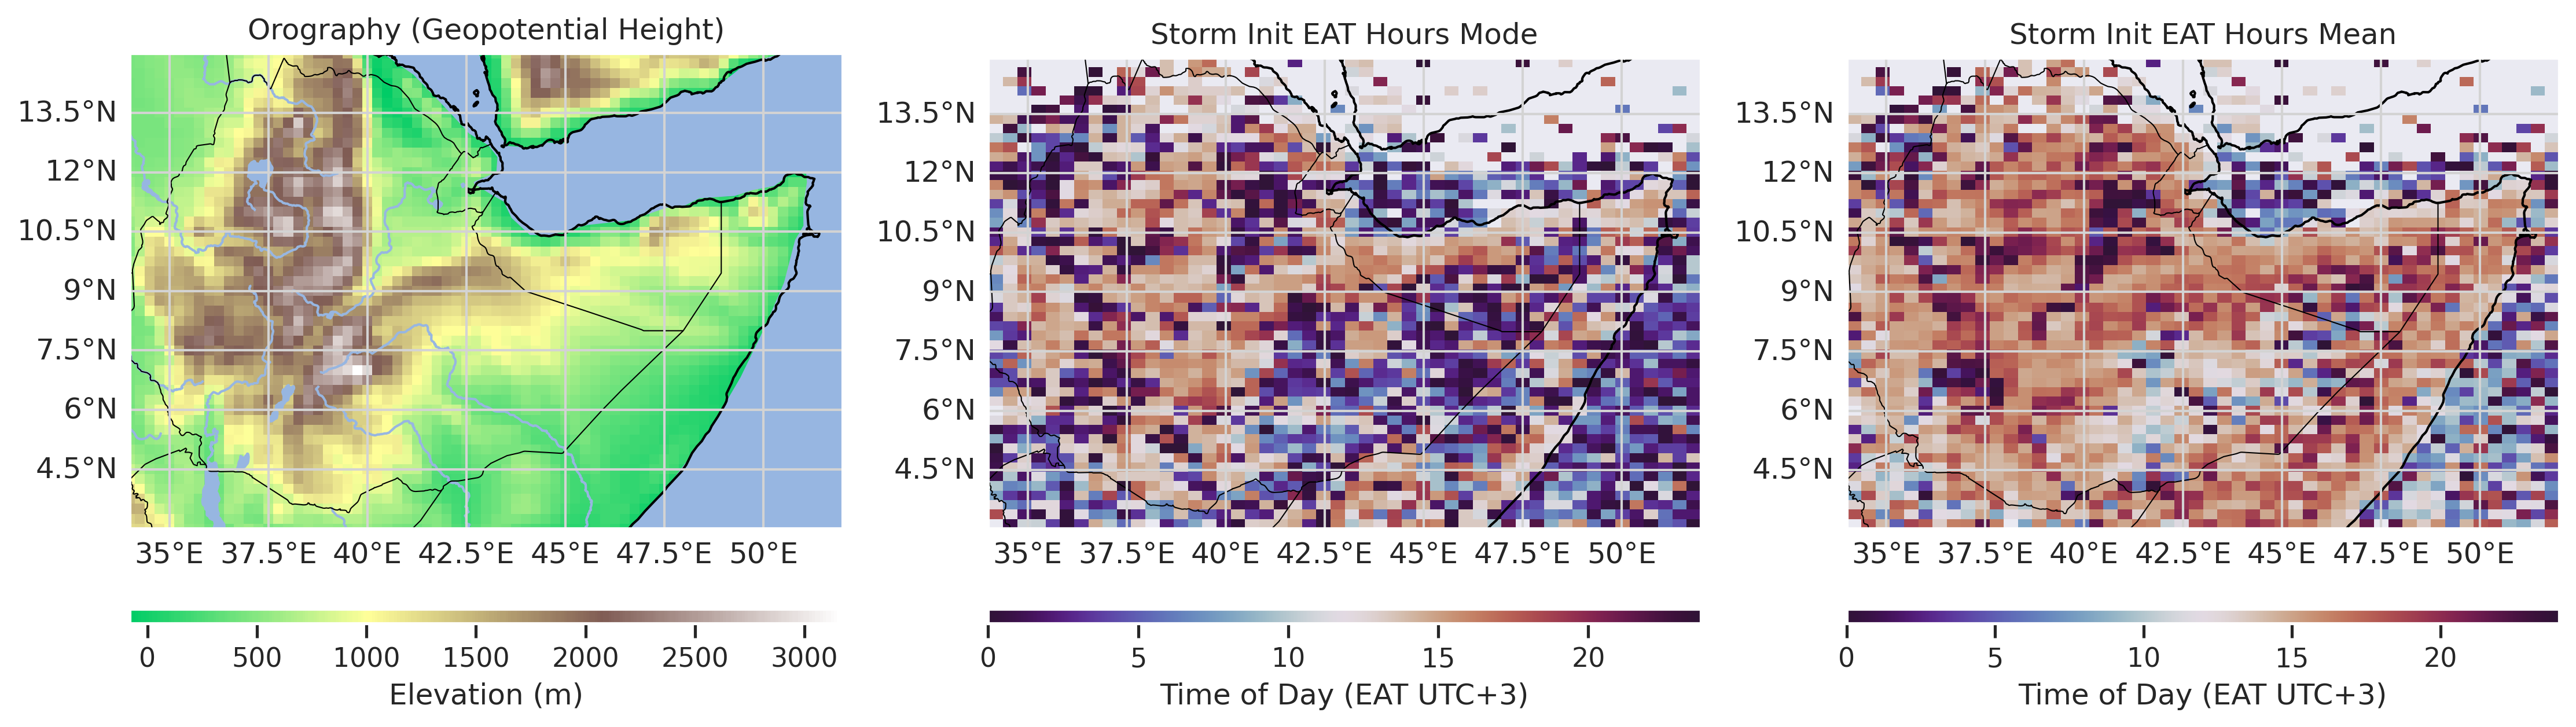
\includegraphics[width=\textwidth]{../figures/generated/exploration/orography_storm_init_eat_hours_mode_mean.png}
    \caption{Storm Genesis Local Time (\acrlong{eat}). Elevation was calculated from \acrshort{era5} geopotential height data.}
    \label{fig:orography_storm_init_eat_hours_mode_mean}
\end{figure}

Finally, Figure \ref{fig:min_bt_over_lifecycle_by_init_type} shows the minimum \acrshort{bt} over the lifecycle of storms, categorised by their initiation type. For this specific analysis, minimum \acrshort{bt} was interpolated over the storm lifecycle and 11 equally spaced points were extracted so as to facilitate comparison across storms of varying durations. Interestingly, on average, storms which initiated over the ocean and during the night both tend to be weaker over the entire storm duration. This dynamic may be picked up by the models and should surface in the importance of features like local time (\texttt{eat\_hours}) and the over land flag (\texttt{over\_land}). 

\begin{figure}[ht]
    \centering
    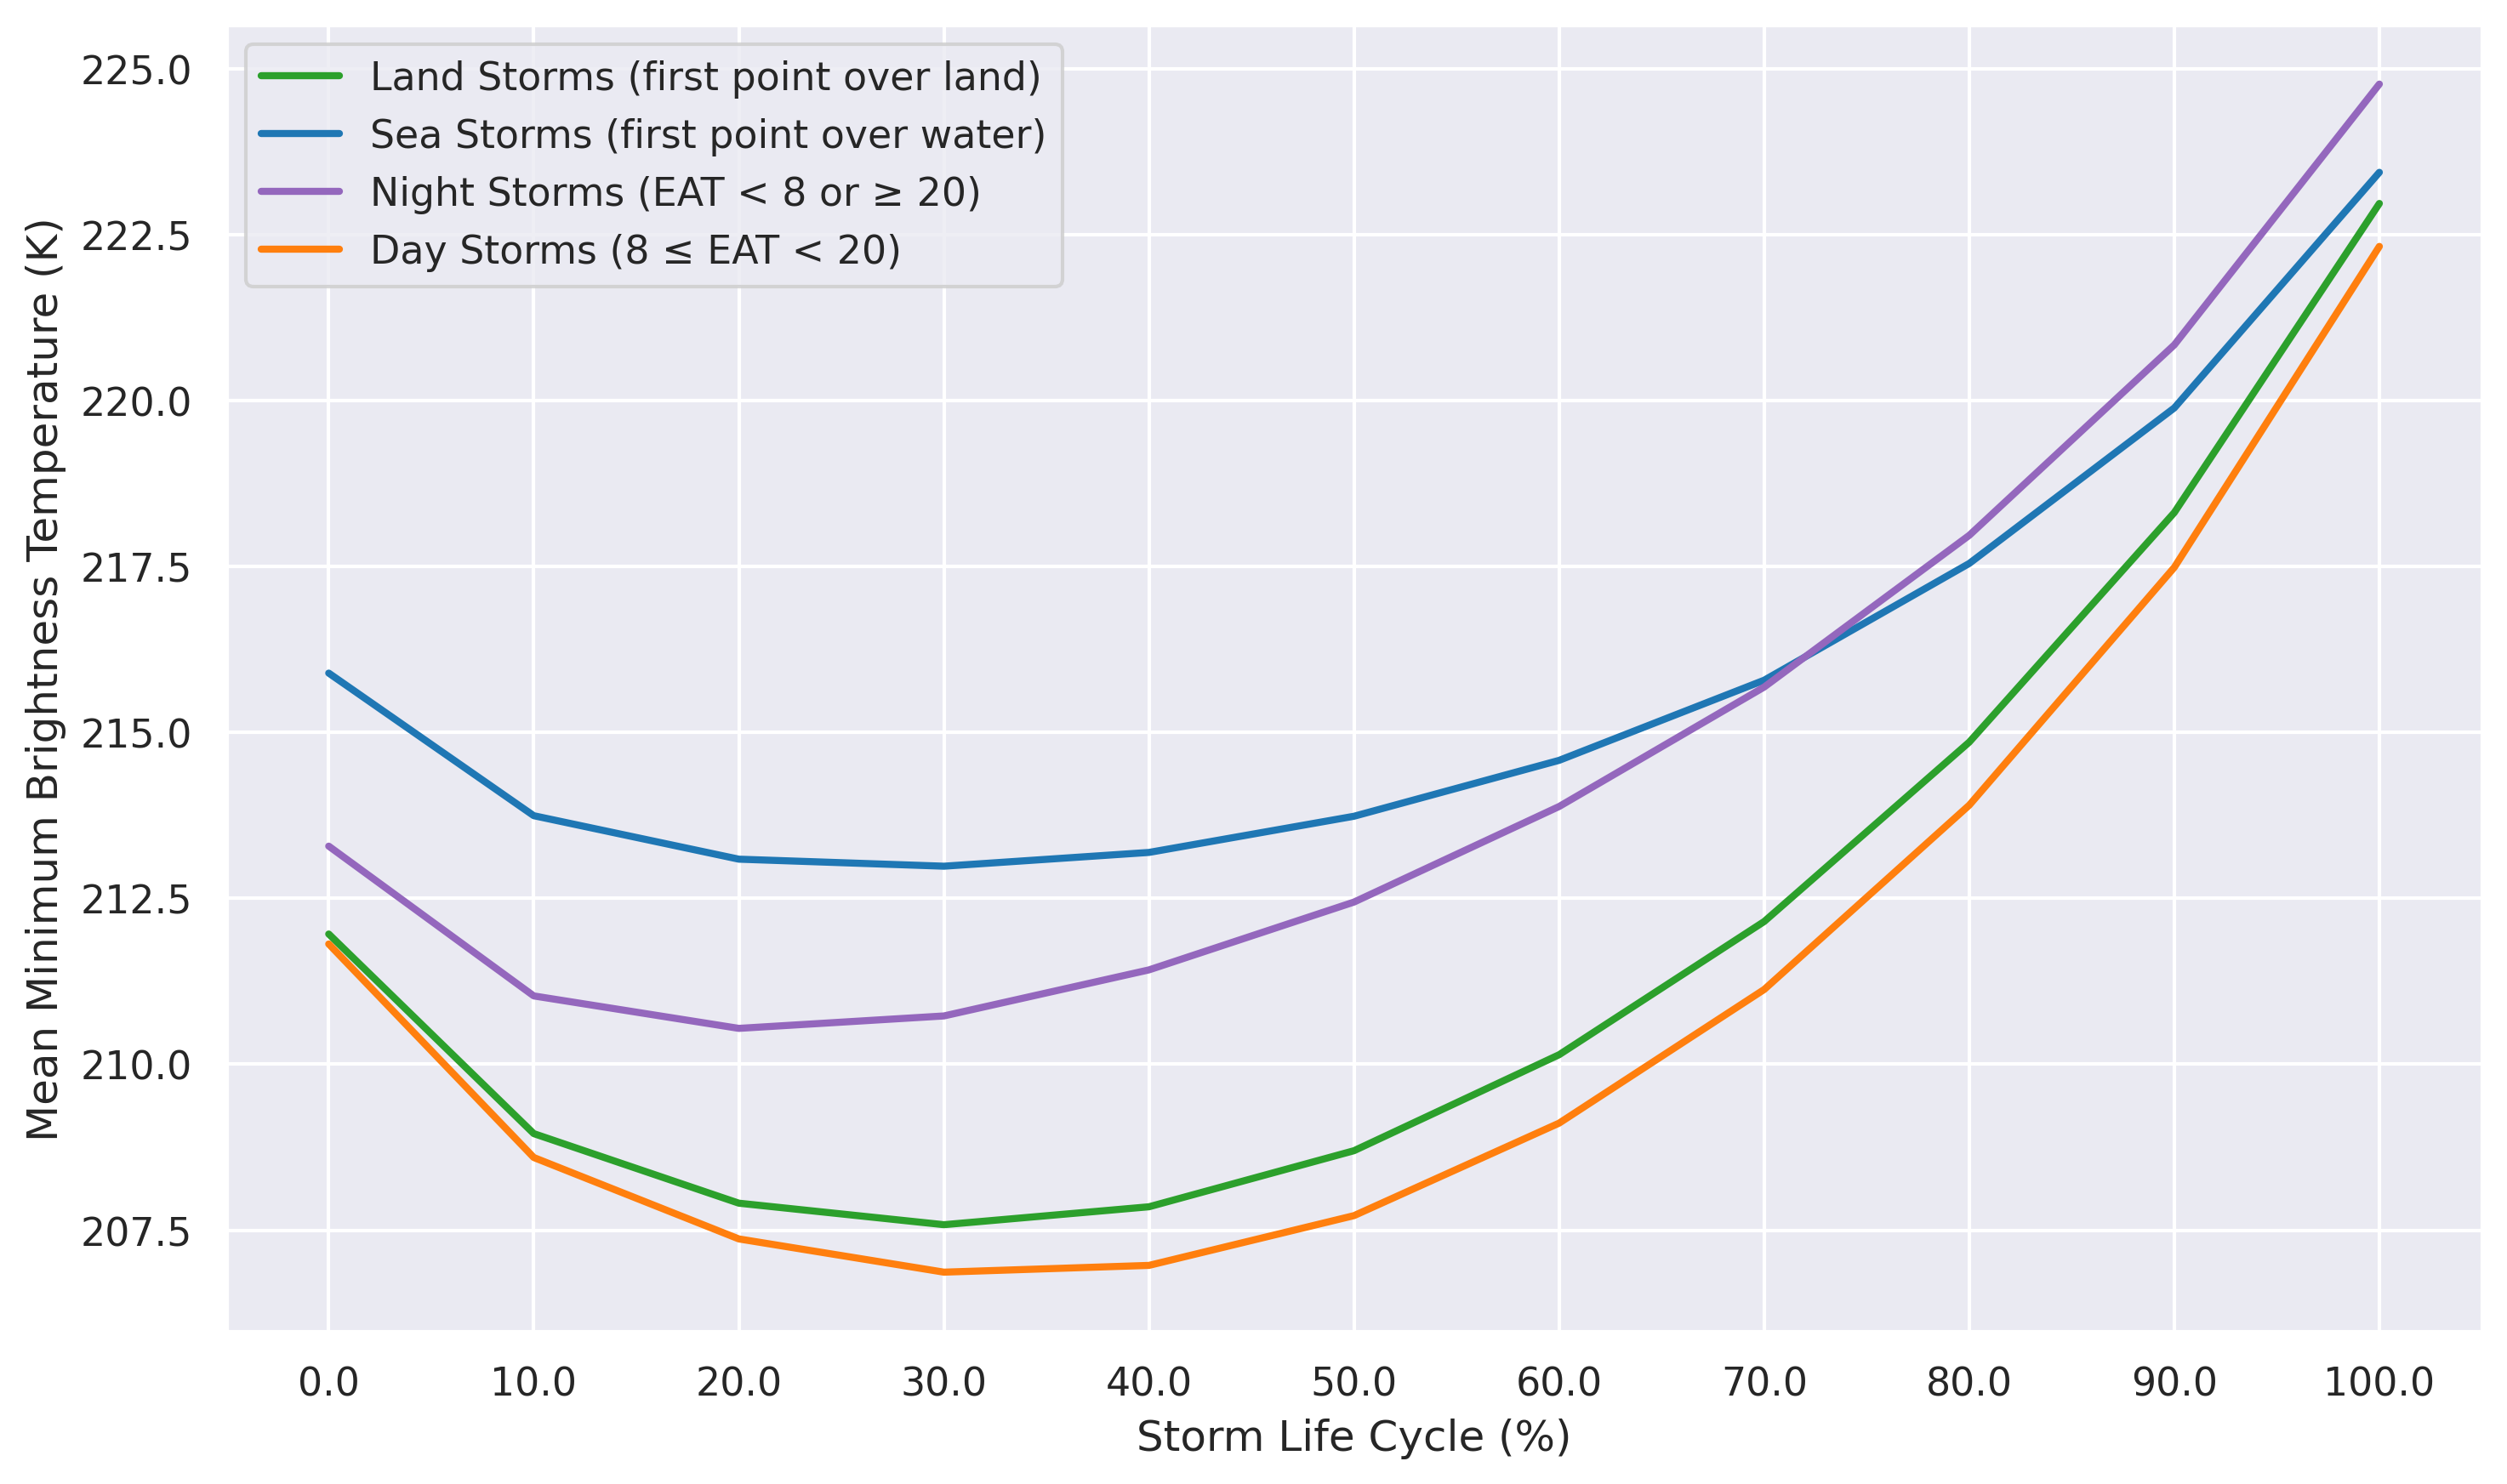
\includegraphics[width=0.5\textwidth]{../figures/generated/exploration/min_bt_over_lifecycle_by_init_type.png}
    \caption{Minimum \acrfull{bt} over the lifecycle of storms, categorised by their initiation type.}
    \label{fig:min_bt_over_lifecycle_by_init_type}
\end{figure}

\section{Predict Storm Aggregate Features}

This following two sections provide an overview of the experimental results obtained from the various predictive tasks outlined in the methodology. The experiments in this section aim to predict the overall characteristics of a storm and assess the predictive power of a storm's initial observation.

\subsection{Storm Maximum Intensity}

Table \ref{tab:storm_max_intensity_results} details the performance metrics for storm maximum intensity prediction across the different experimental setups. Note that the target predictand was \texttt{storm\_min\_bt} so lower values are stronger. The result metrics indicate that ERA5 features alone perform comparably to using all available features, suggesting that the meteorological variables capture most of the relevant information for predicting storm maximum intensity. However, restricting the models to only the first observation points leads to a substantial drop in performance. Subsequently, further explainability analysis will only focus on the all observations models.

\begin{table}[ht]
\centering
\caption{Experiment results for storm maximum intensity prediction}
\label{tab:storm_max_intensity_results}
\begin{tabular}{lccccc}
\hline
\textbf{Experiment} & \multicolumn{2}{c}{\textbf{RMSE}} & \multicolumn{2}{c}{\textbf{Target Std}} & \textbf{Actual vs. Predicted $R^2$} \\
\cline{2-5}
 & \textbf{All} & \textbf{First pts} & \textbf{All} & \textbf{First pts} &  \\
\hline
All              & 2.7610 & 4.4872 & 9.1679 & 8.8540 & 0.9098 \\
\acrshort{era5}             & 2.7503 & 4.1075 & 9.1679 & 8.8540 & 0.9134 \\
All First Points & \multicolumn{2}{c}{7.2265} & \multicolumn{2}{c}{8.9432} & 0.3478 \\
\acrshort{era5} First Points & \multicolumn{2}{c}{7.4673} & \multicolumn{2}{c}{8.9432} & 0.3034 \\
\hline
\end{tabular}
\end{table}

\begin{figure}[ht]
    \centering
    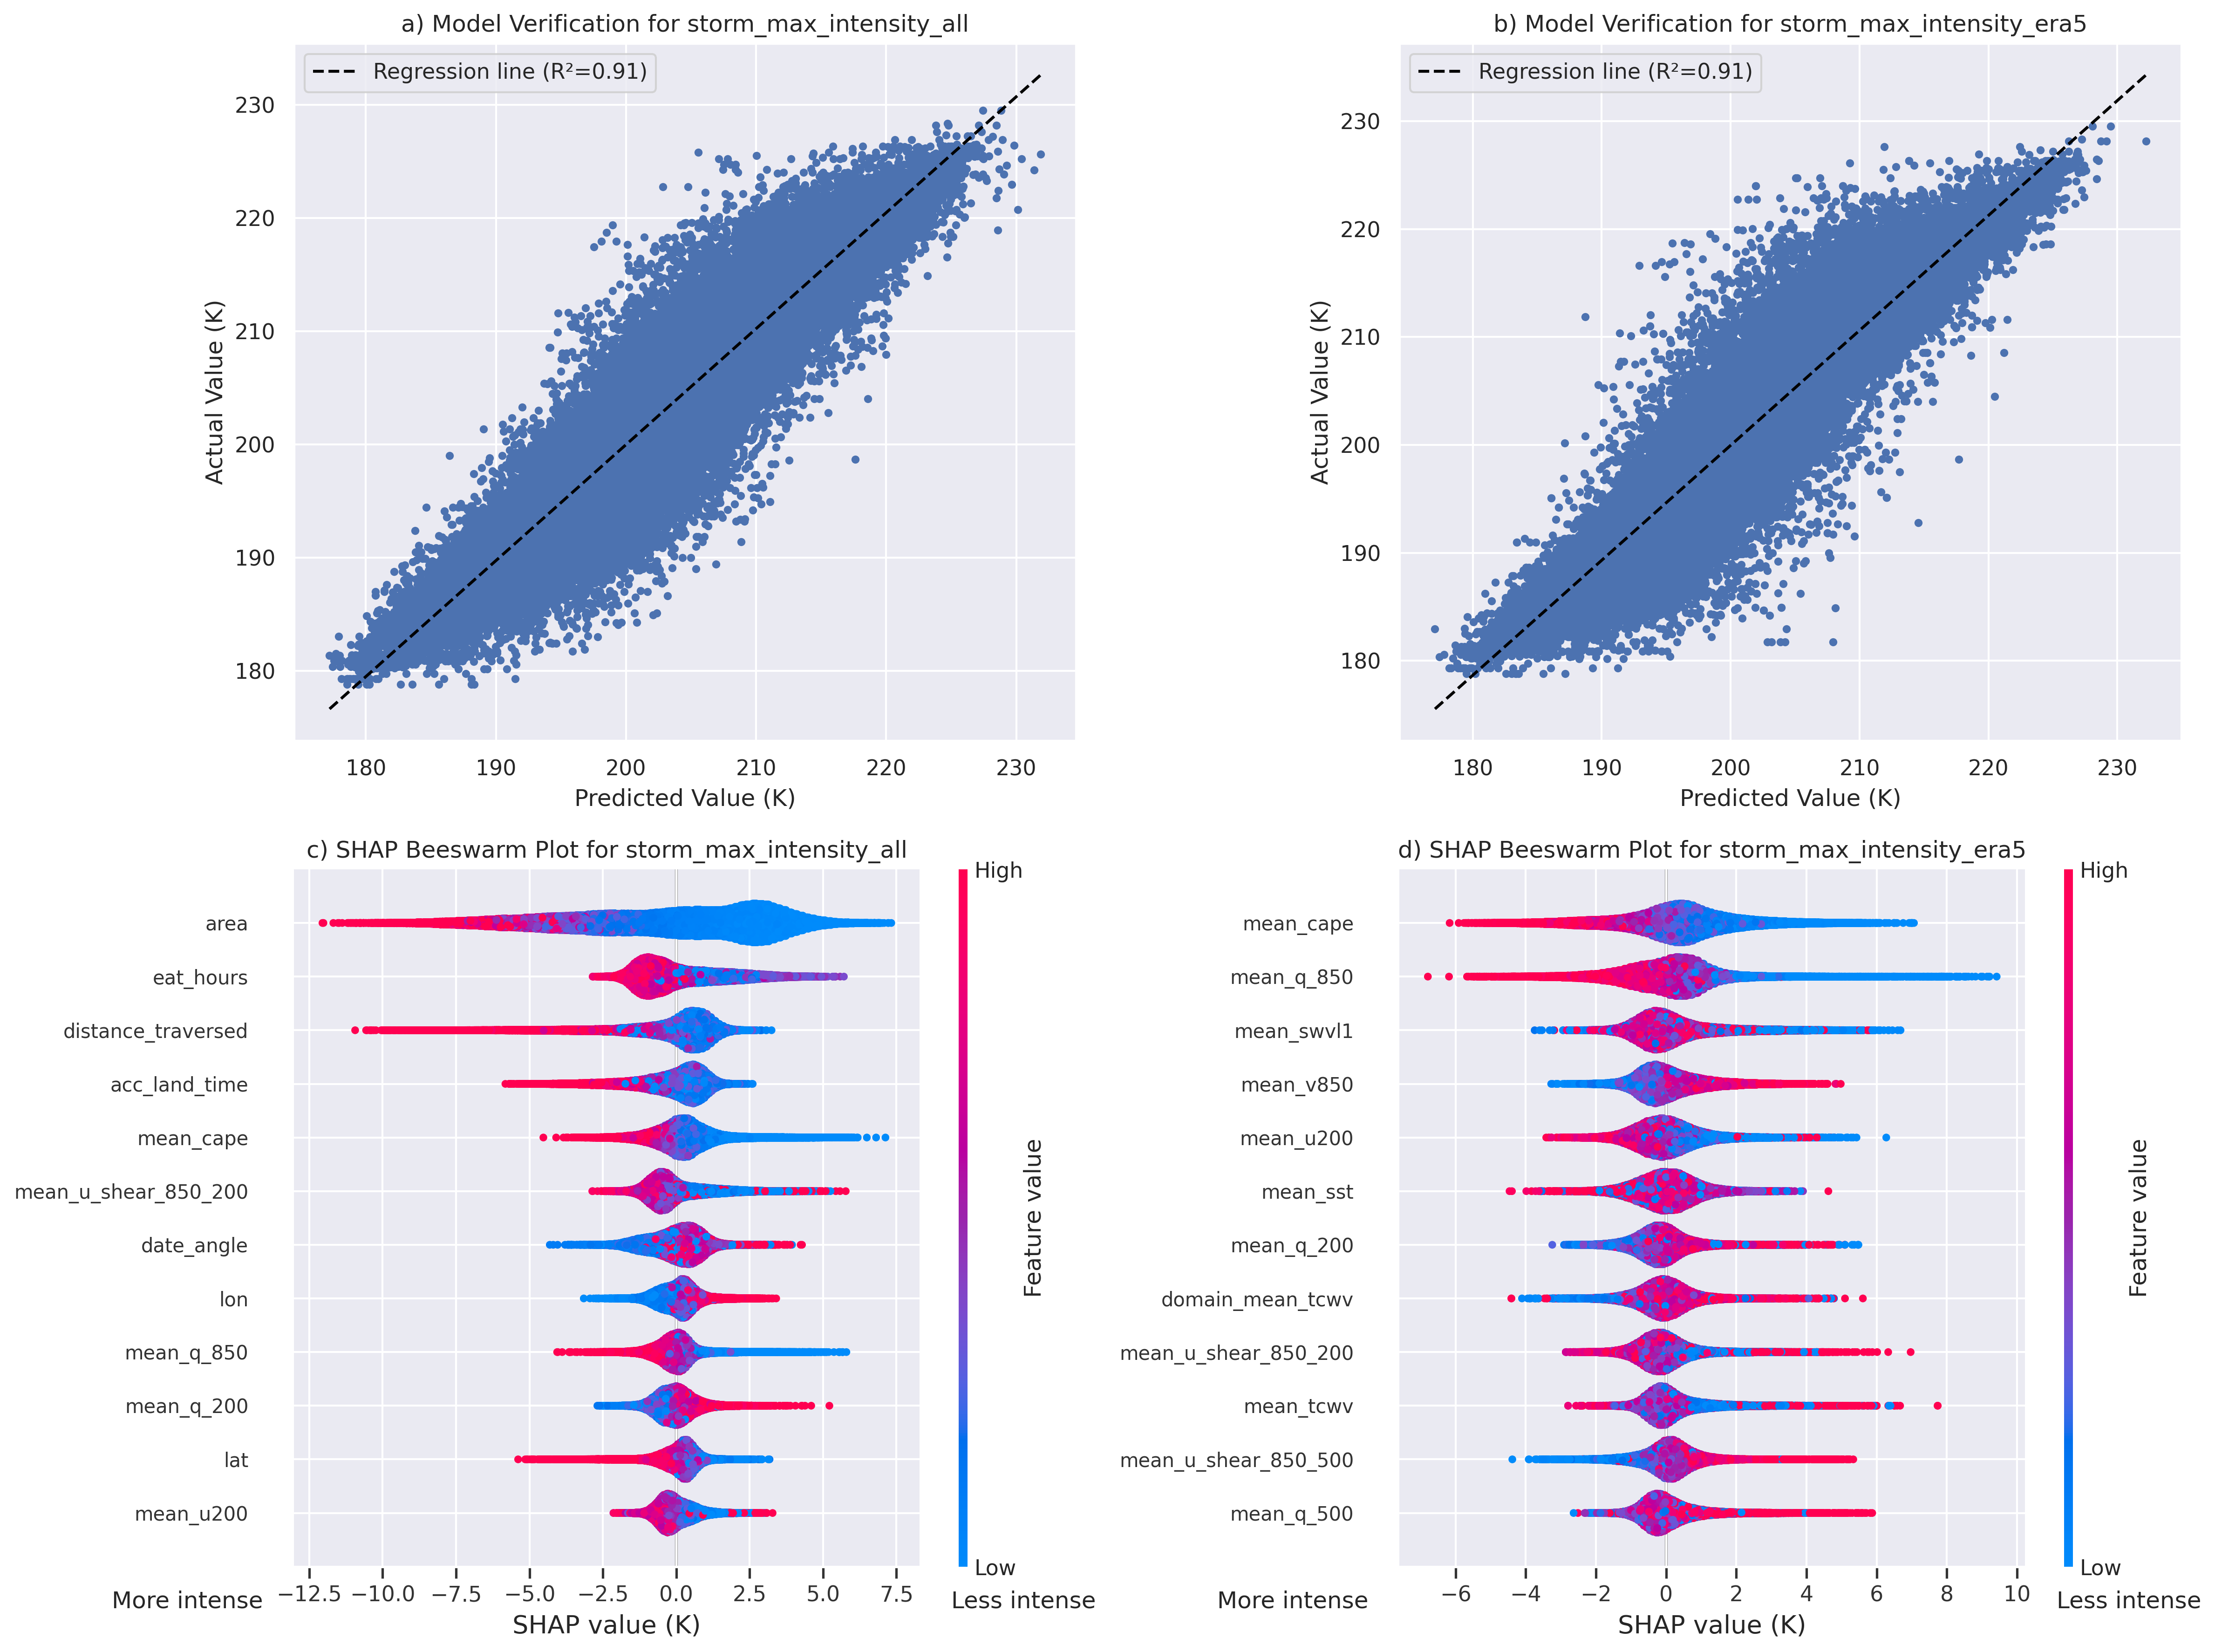
\includegraphics[width=0.8\textwidth]{../figures/generated/experiments/storm_max_intensity/storm_max_intensity_summary.png}
    \caption{Comparison of performance and top features for storm maximum intensity.}
    \label{fig:storm_max_intensity_summary}
\end{figure}

Figure \ref{fig:storm_max_intensity_summary} presents a detailed comparison of the model performance and the most influential features for predicting storm maximum intensity using all features versus \acrshort{era5} only. Notably, for the all features model, only one meteorological variable appears among the top five most important features. The results of the all features model also reveal a weak but present diurnal cycle, with stronger storms tending to develop in the late evening. Across both models, \acrshort{cape} consistently emerges as the most important meteorological factor.

Particularly striking for these models is that the importance of low-level meridional winds changes with time of day, date, and location. Figure \ref{fig:storm_max_intensity_era5_shap_mean_v850_map_by_month} illustrates this variability over the study region throughout the year. During the summer months, the influence is predominantly positive over the Somali coastal plains and negative over the Ethiopian Highlands, indicating a diminishing effect on storm intensity in the southeast. Conversely, in the winter months, the influence tends to be negative or neutral over the entire domain.

\begin{figure}[ht]
    \centering
    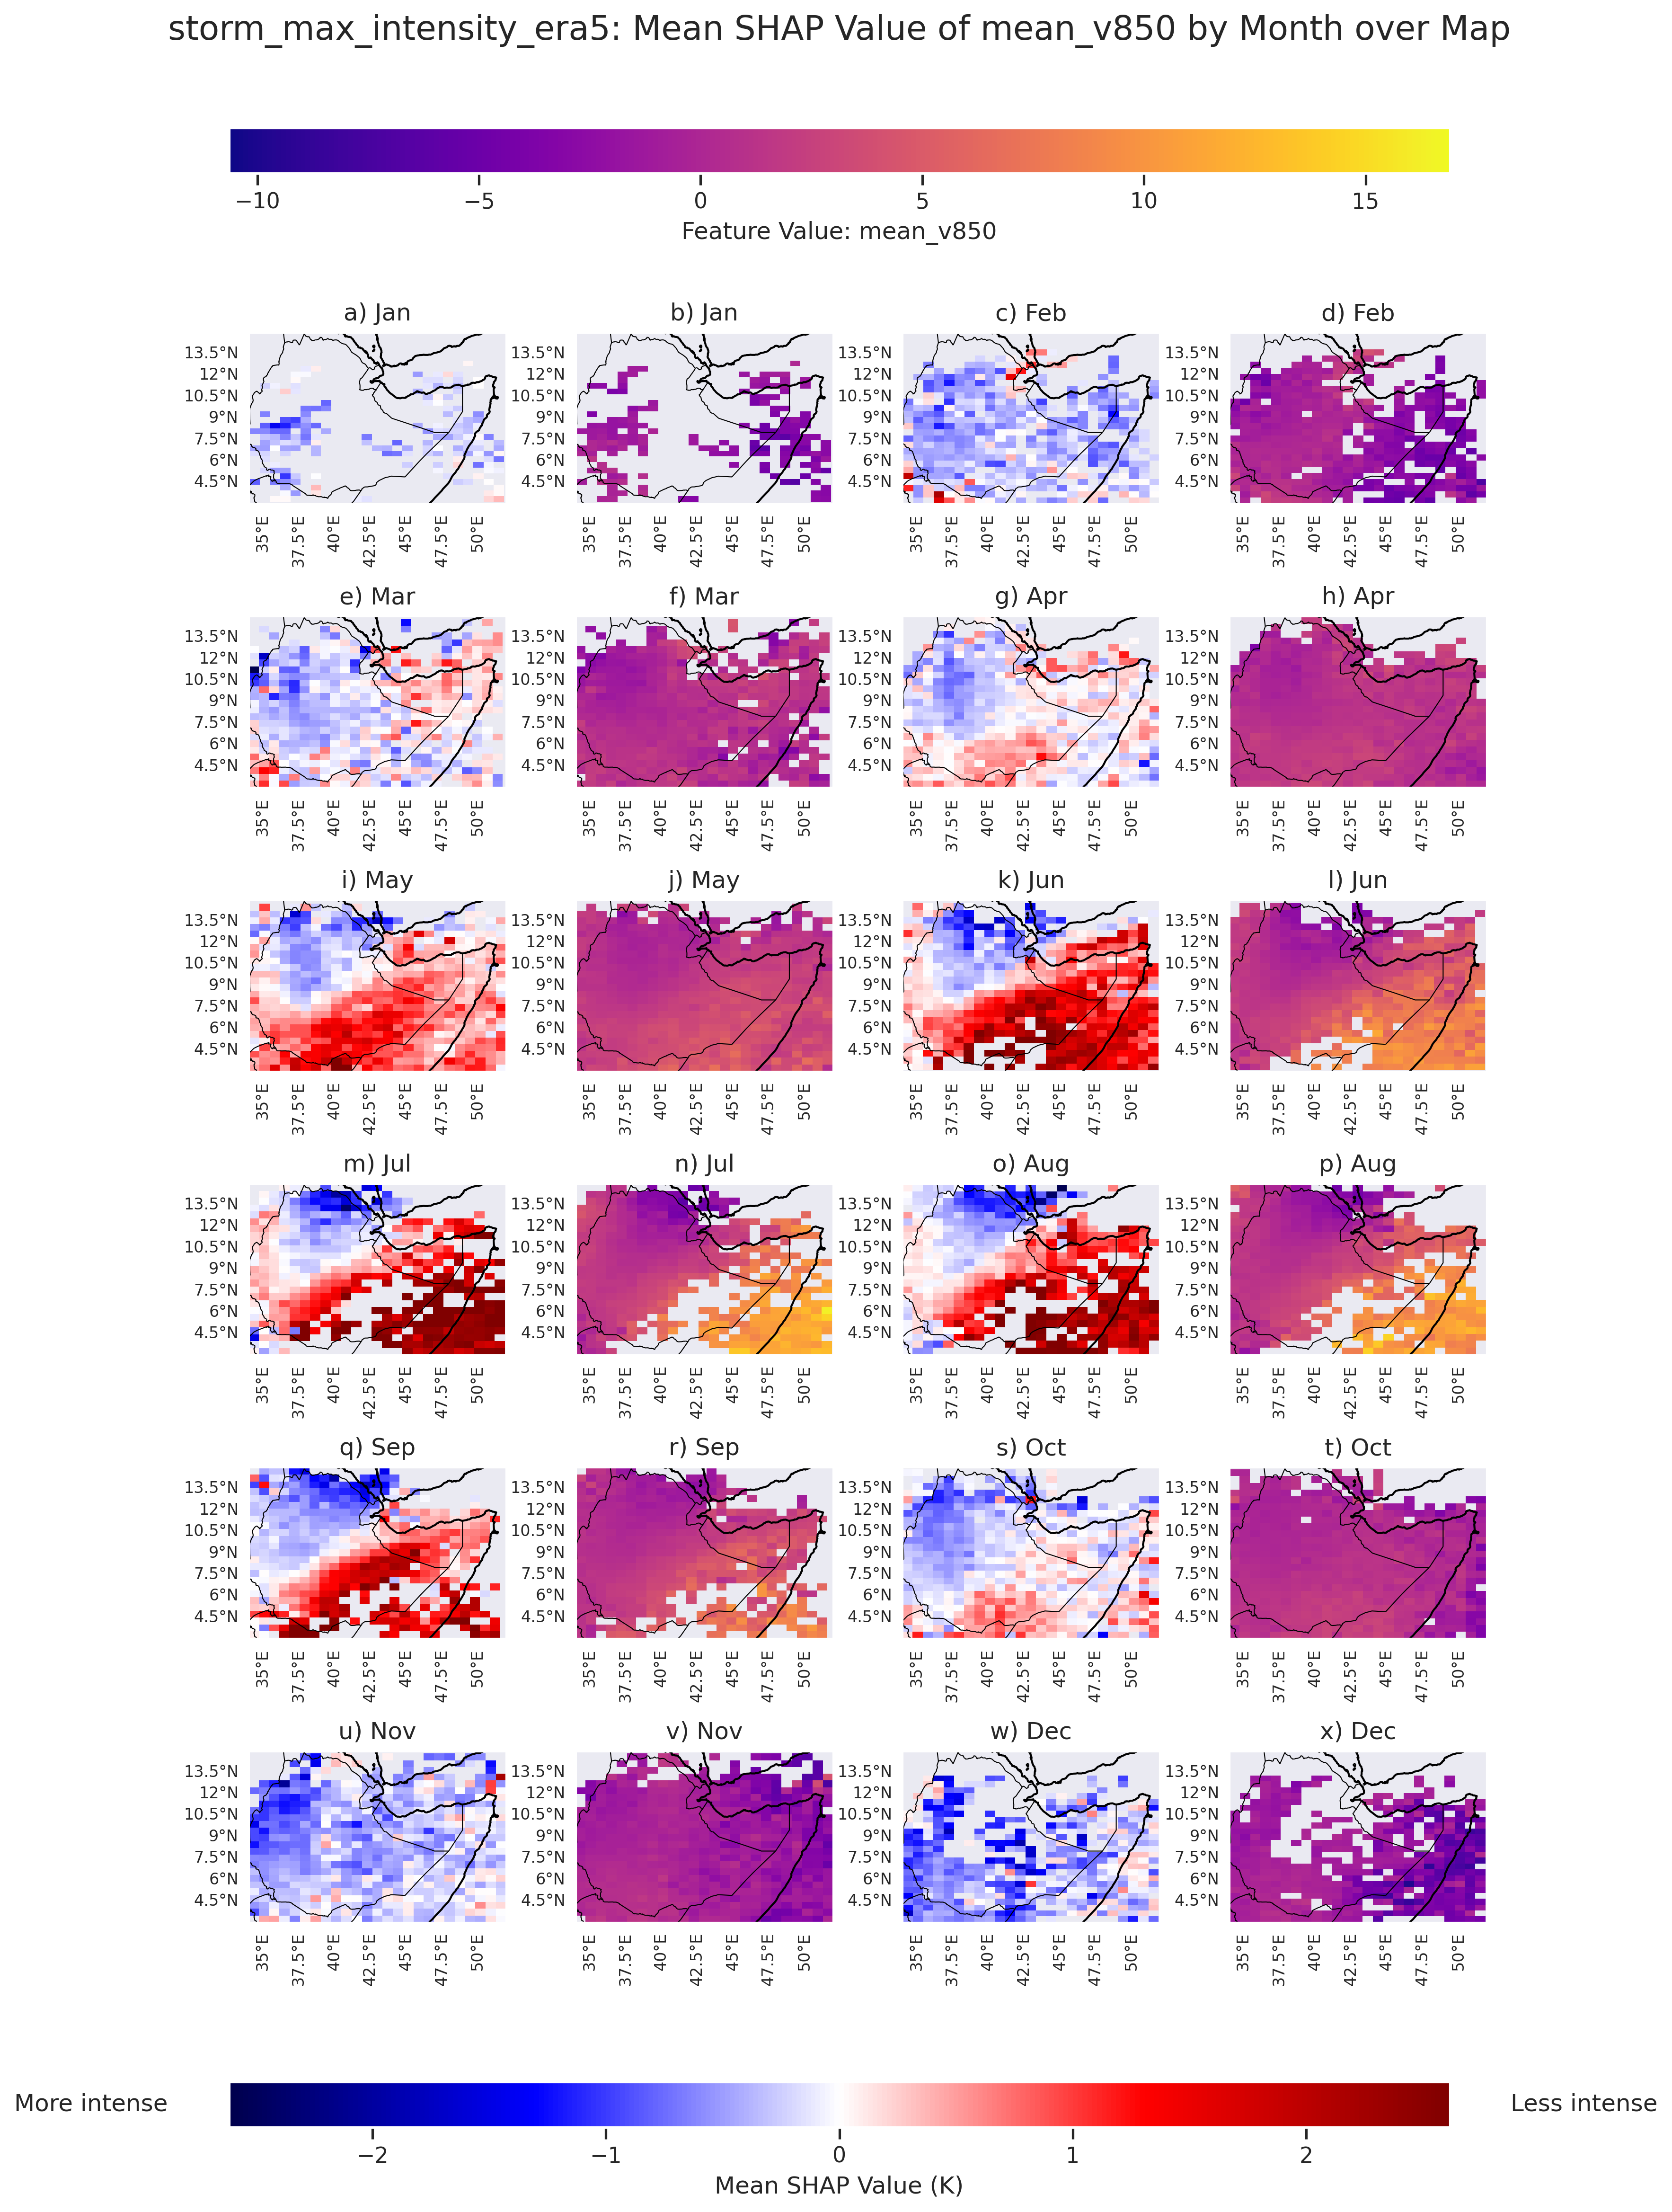
\includegraphics[width=0.8\textwidth]{../figures/generated/experiments/storm_max_intensity/geographic_corr/storm_max_intensity_era5_shap_mean_v850_map_by_month.png}
    \caption{Mean SHAP values for 850 hPa meridional wind over East Africa by month for storm maximum intensity prediction using ERA5 features.}
    \label{fig:storm_max_intensity_era5_shap_mean_v850_map_by_month}
\end{figure}
\todo{can remove plot title here later. kept it for easier exploration of all the figures i generated}

\clearpage
\subsection{Storm Direction}

Table \ref{tab:storm_direction_results} details the performance metrics for storm direction prediction across different experimental setups as specified in the methodology. Again, due to the poor performance of the first points only models, further explainability analysis will focus on the all observations models.

\begin{table}[ht]
\centering
\caption{Experiment results for storm direction prediction}
\label{tab:storm_direction_results}
\begin{tabular}{lccccc}
\hline
\textbf{Experiment} & \multicolumn{2}{c}{\textbf{RMSE}} & \multicolumn{2}{c}{\textbf{Target Std}} & \textbf{Actual vs. Predicted $R^2$} \\
\cline{2-5}
 & \textbf{All} & \textbf{First pts} & \textbf{All} & \textbf{First pts} &  \\
\hline
All              & 20.6609 & 35.0730 & 75.7506 & 76.8966 & 0.9281 \\
\acrshort{era5}             & 18.2928 & 31.6709 & 75.7506 & 76.8966 & 0.9437 \\
All First Points & \multicolumn{2}{c}{60.7651} & \multicolumn{2}{c}{78.7438} & 0.4047 \\
\acrshort{era5} First Points & \multicolumn{2}{c}{61.4484} & \multicolumn{2}{c}{78.7438} & 0.3912 \\
\hline
\end{tabular}
\end{table}

For better context in interpreting the meaning of the \acrshort{shap} values, Figure \ref{fig:storm_cardinal_directions_distribution} shows the distribution of storm cardinal directions in the dataset. The distribution indicates that the majority of storms move in a westerly direction and indeed the mean storm direction is approximately \ang{258}. Thus, generally for this experiment, positive \acrshort{shap} values can be interpreted as shifting the predicted storm direction northward, while negative values indicate a southward shift.

\begin{figure}[ht]
    \centering
    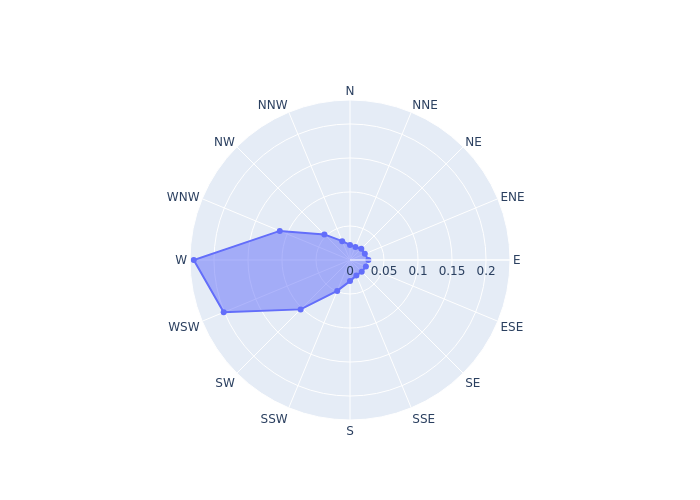
\includegraphics[width=0.6\textwidth]{../figures/generated/exploration/storm_cardinal_directions_distribution.png}
    \caption{Distribution of storm cardinal directions in the dataset.}
    \label{fig:storm_cardinal_directions_distribution}
\end{figure}

\begin{figure}[ht]
    \centering
    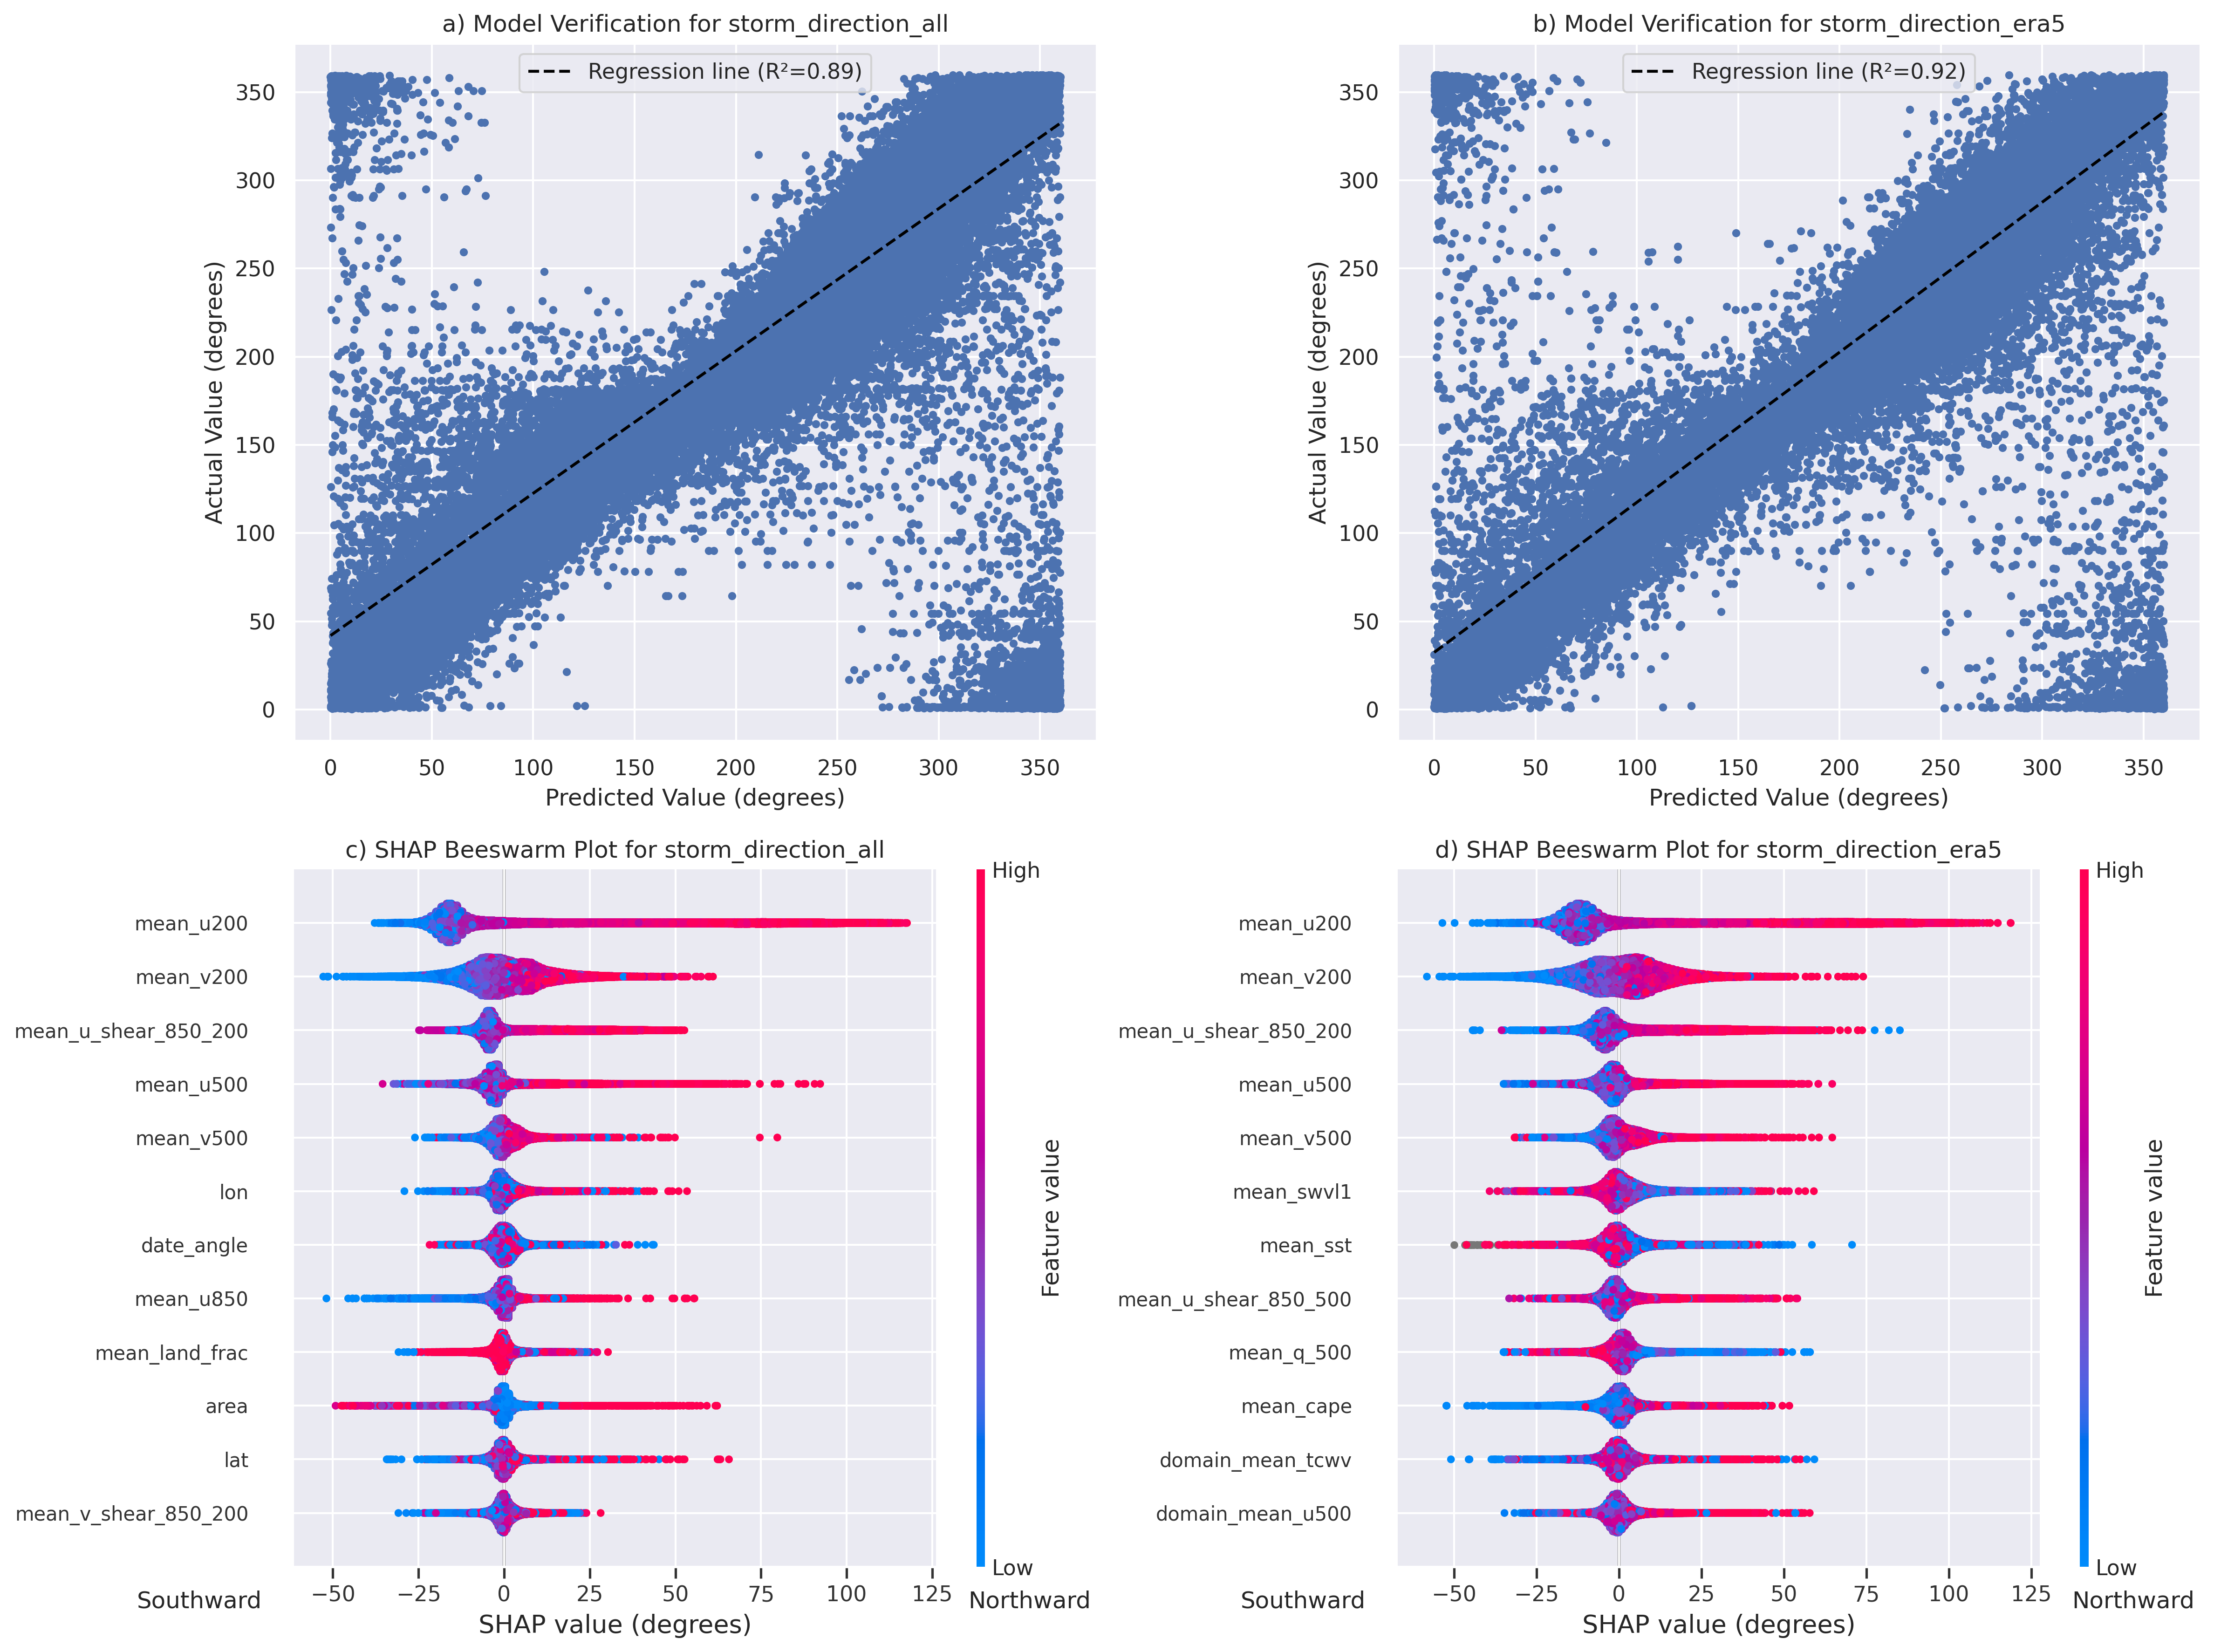
\includegraphics[width=0.8\textwidth]{../figures/generated/experiments/storm_direction/storm_direction_summary.png}
    \caption{Comparison of performance and top features for storm direction.}
    \label{fig:storm_direction_summary}
\end{figure}

Low-level zonal winds are by far the most important factor for predicting storm direction, as shown in Figure \ref{fig:storm_direction_summary} c) and d). Positive values of \texttt{mean\_u850} (westerly winds) tend to shift the predicted storm direction eastward. \texttt{eat\_hours} does not appear in the top 12 features indicating that diurnal cycle is not a significant factor for storm direction. Mid-level zonal winds also appear to be important, as shown in Figure \ref{fig:storm_direction_all_shap_mean_u500_map_by_month}. The influence of these winds varies with location and time of year. During the summer months, the influence is predominantly negative over the Somali coastal plains and positive over the Ethiopian Highlands. During the end of the year, the influence appears mostly neutral over the entire domain. However, in the spring, the influence is the summer influence but mirrored horizontally, with negative values over the Gulf of Aden and positive values on the Ethiopian border with South Sudan and Kenya.

\begin{figure}[ht]
    \centering
    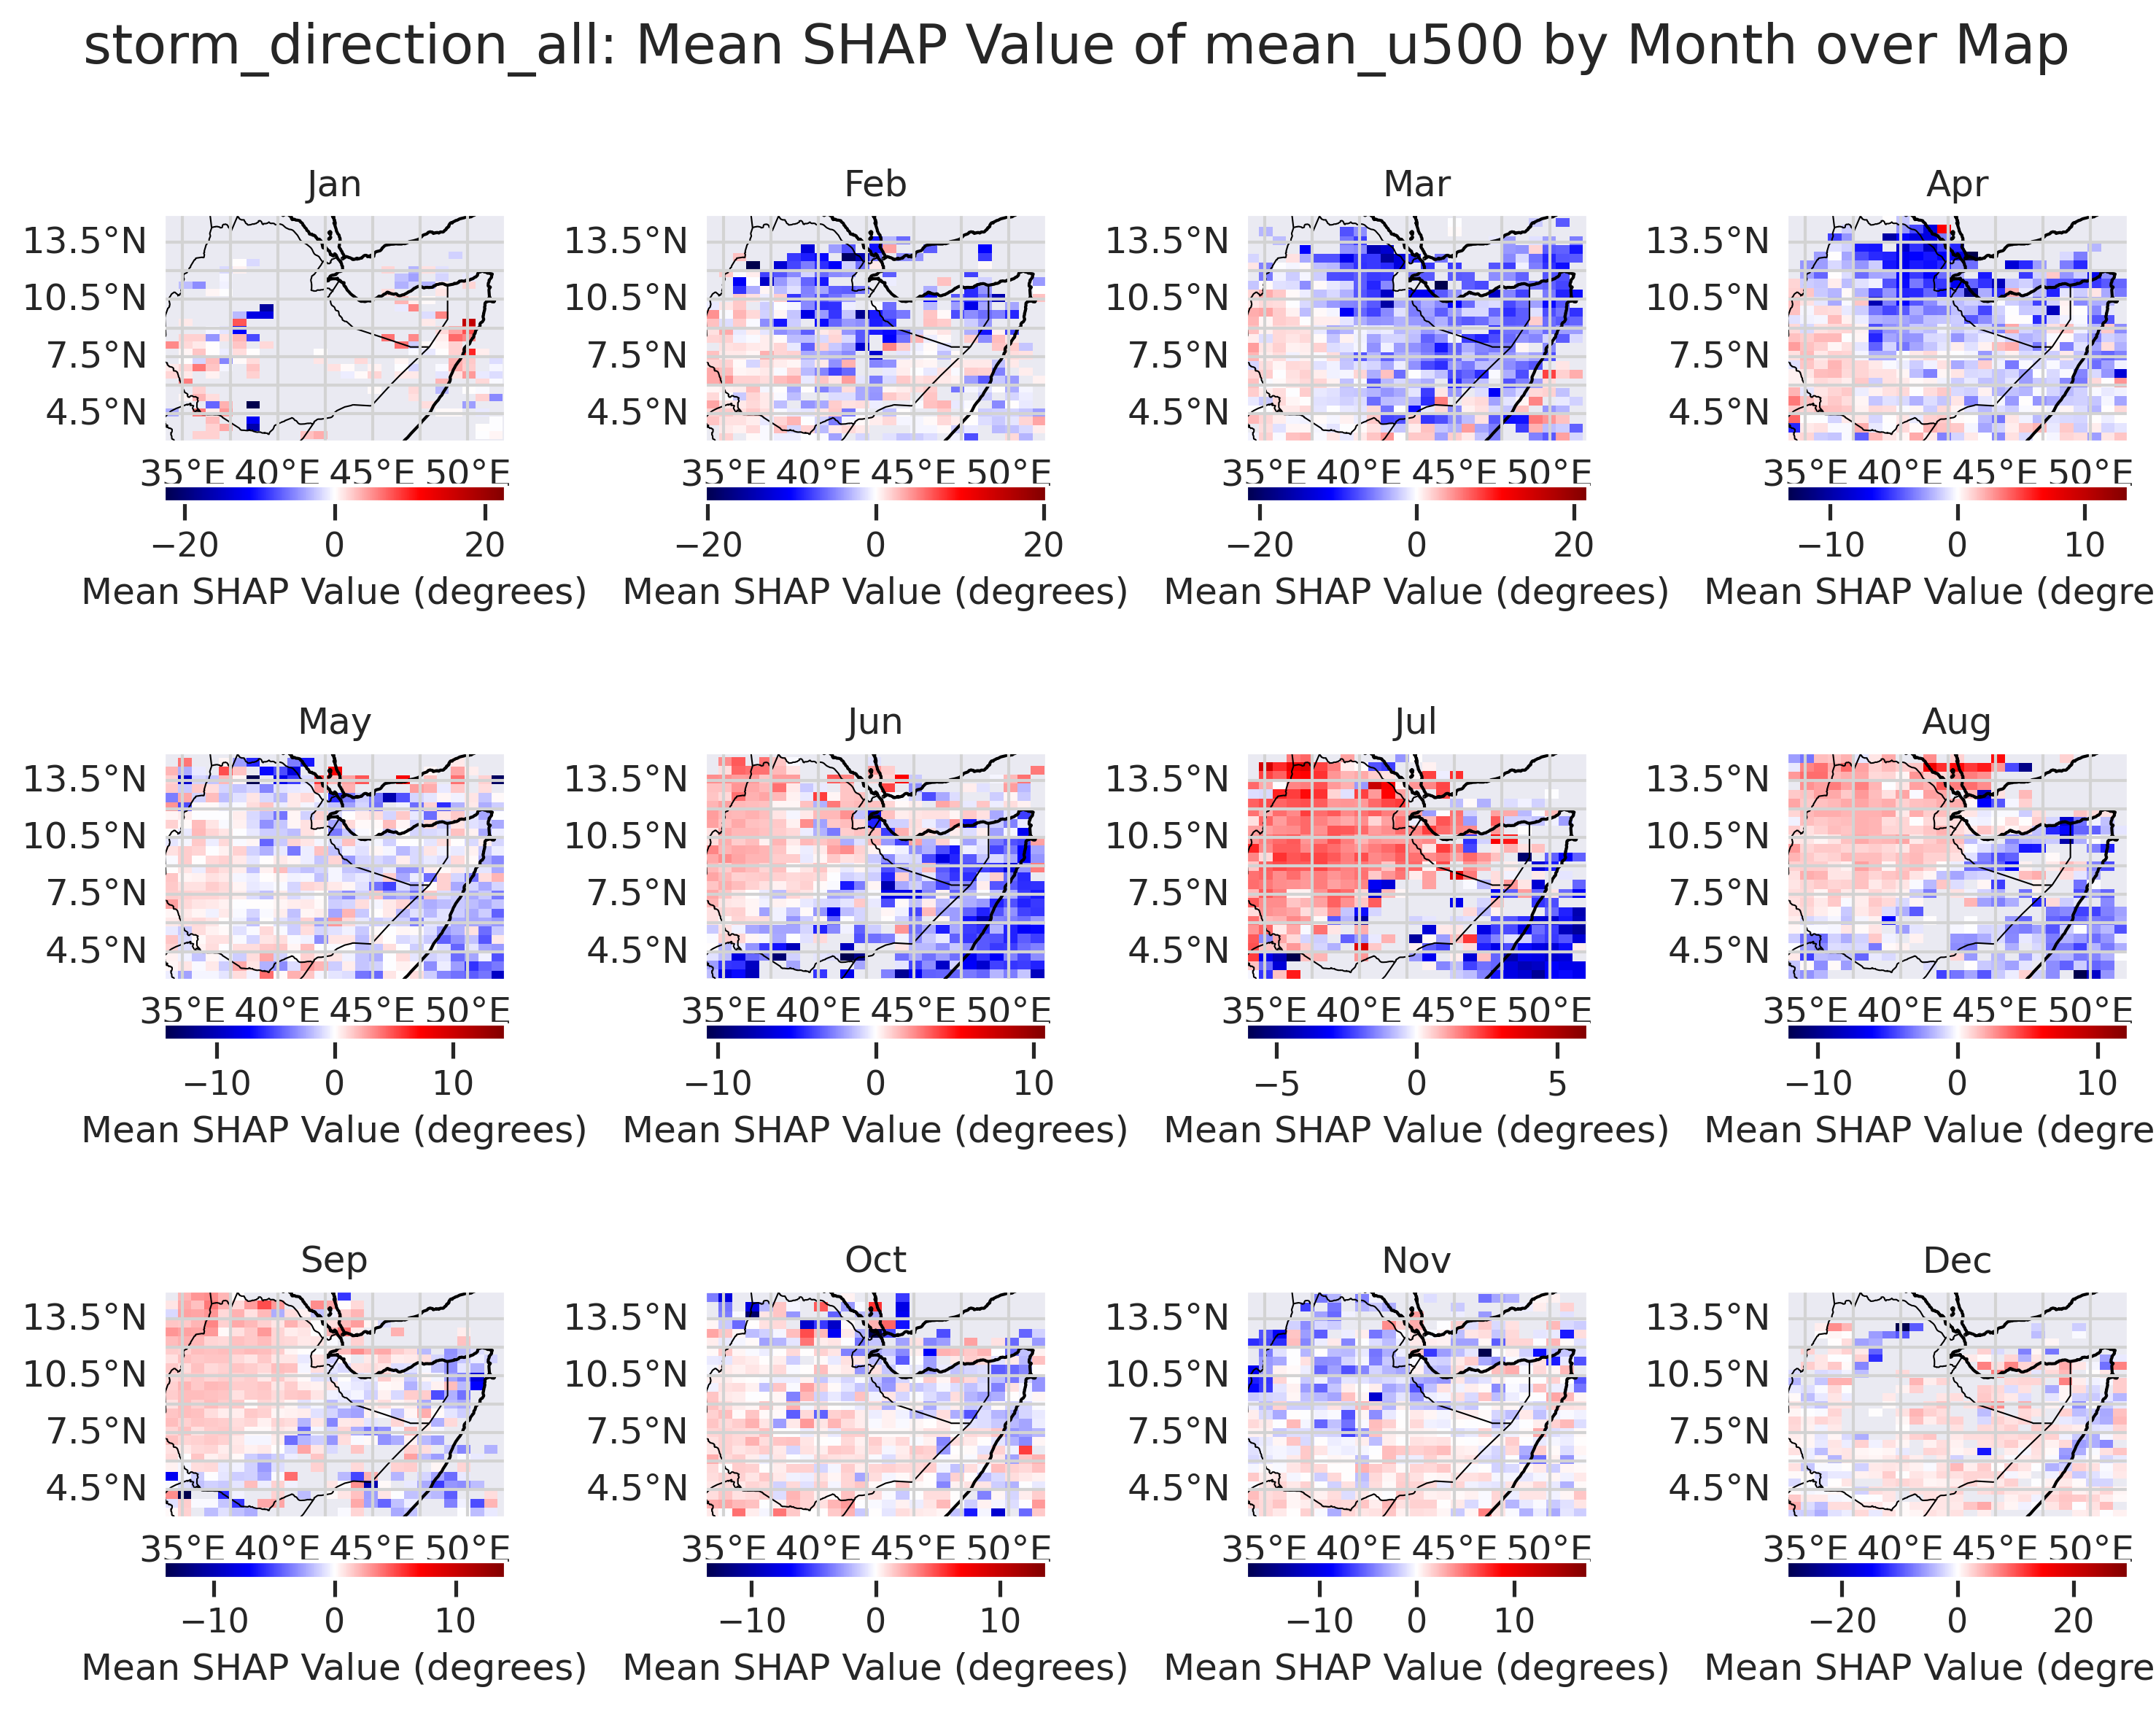
\includegraphics[width=0.8\textwidth]{../figures/generated/experiments/storm_direction/geographic_corr/storm_direction_all_shap_mean_u500_map_by_month.png}
    \caption{Mean SHAP values for 500 hPa zonal wind over East Africa by month for storm direction prediction using all features.}
    \label{fig:storm_direction_all_shap_mean_u500_map_by_month}
\end{figure}

\clearpage
\section{Predict Immediate Characteristics at an Observation}

These experiments aim to predict the immediate characteristics of a storm based on its current observation and Table \ref{tab:obs_experiment_results} shows performance metrics of the models. Unfortunately, \acrshort{xgb} struggled to accurately predict the next direction and distance of the storm, as indicated by the \acrshort{rmse} values being only slightly lower than the standard deviation of the target variable and the resulting low R-squared values between the predicted and actual values. As such, no further explainability analysis will be conducted on those experiments. However, possible reasons for this poor performance and future directions for improvement are discussed in Chapter \ref{ch:discuss}.

\begin{table}[h!]
\centering
\caption{Immediate Characteristic at Observation Results}
\label{tab:obs_experiment_results}
\begin{tabular}{lccc}
\hline
\textbf{Experiment} & \textbf{Test RMSE} & \textbf{Target Std} & \textbf{R-squared} \\
\hline
Intensification All     & 2.8149  & 4.4840  & 0.6073 \\
Intensification \acrshort{era5}    & 3.0828  & 4.4840  & 0.5278 \\
Direction All     & 72.8590 & 86.4541 & 0.2898 \\
Direction \acrshort{era5}     & 74.4878 & 86.4541 & 0.2577 \\
Distance All      & 12.0634 & 13.1260 & 0.1559 \\
Distance \acrshort{era5}     & 12.6901 & 13.1260 & 0.0656 \\
Precipitation All       & 0.0488  & 0.1835  & 0.9296 \\
Precipitation \acrshort{era5}      & 0.0851  & 0.1835  & 0.7887 \\
\hline
\end{tabular}
\end{table}

\clearpage
\subsection{Intensification}

Although the \acrshort{rmse} of the models are acceptable, it is evident that the both models generally tend to underpredict intensification and weakening as shown in Figure \ref{fig:obs_intensification_summary}.

\begin{figure}[ht]
    \centering
    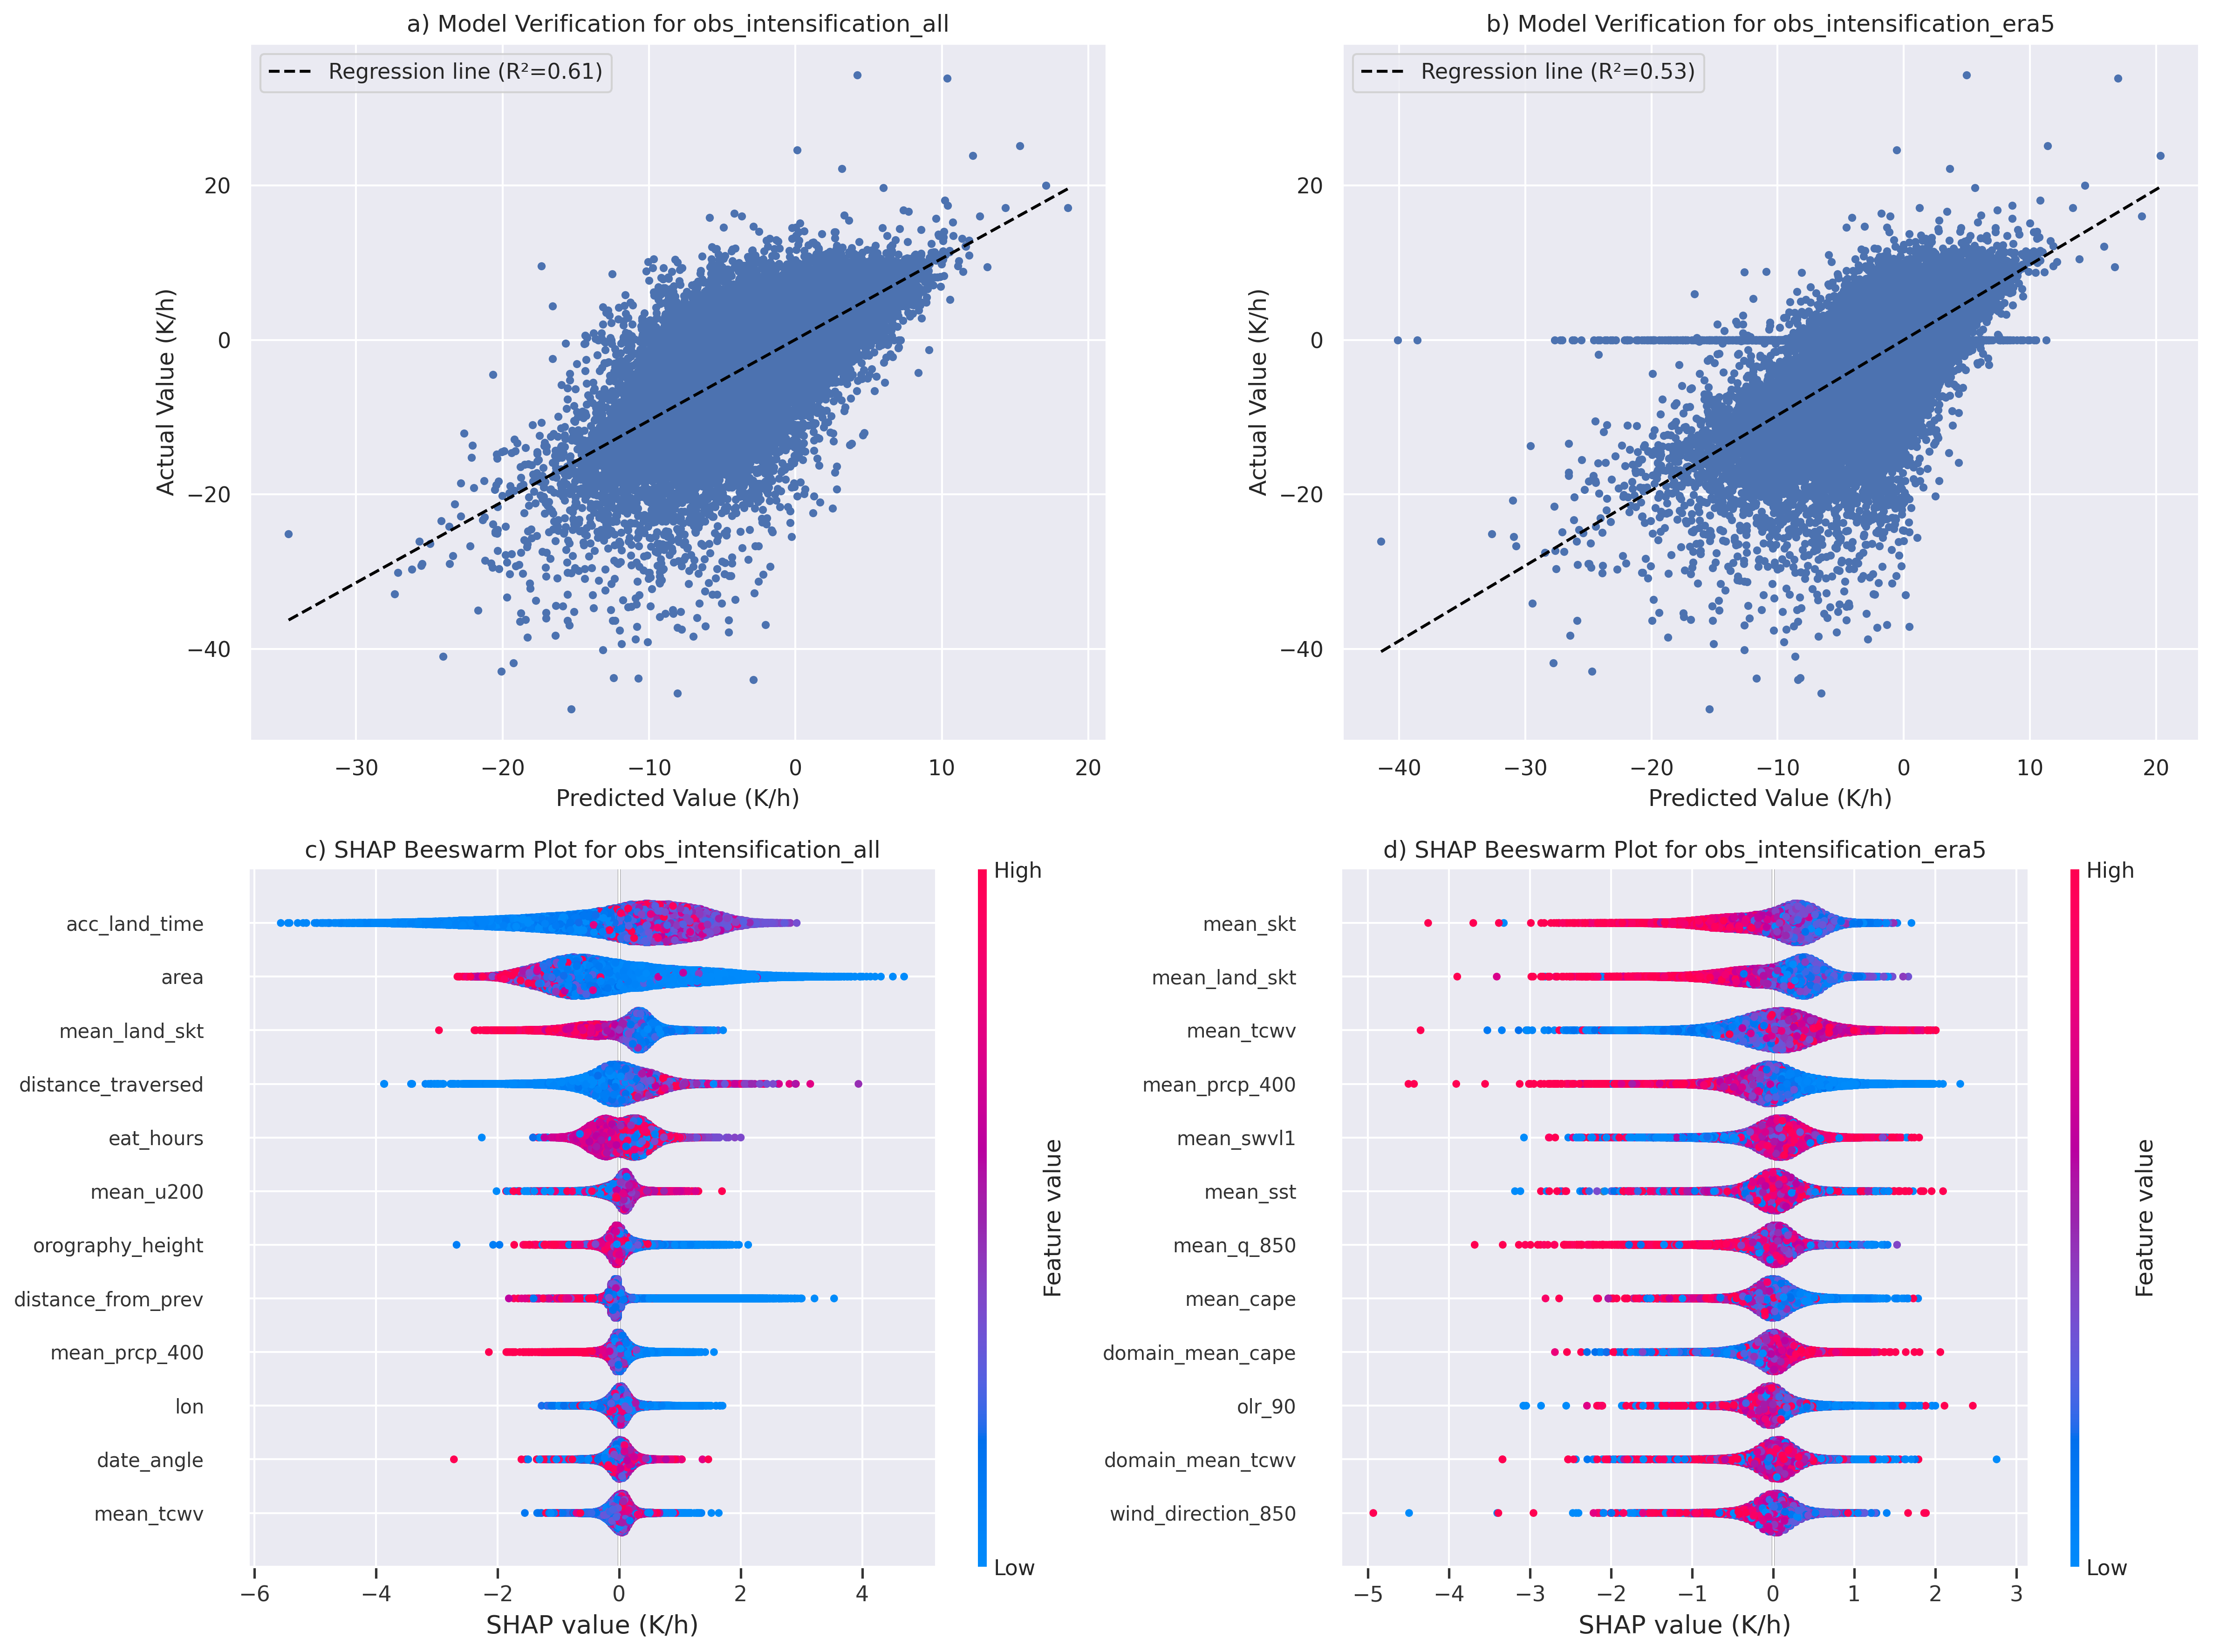
\includegraphics[width=\textwidth]{../figures/generated/experiments/obs_intensification/obs_intensification_summary.png}
    \caption{Comparison of performance and top features for intensification.}
    \label{fig:obs_intensification_summary}
\end{figure}

As for the feature contributions, surface characteristics seem to be particularly important. In the \acrshort{era5} model, land skin, sea surface, and overall skin temperature all appear in the top ten features. Across both models, high land skin temperature consistently emerges as an important factor for intensification. Storms also tend to intensify more when they spend longer periods over the ocean. As for other meteorological variables, in contrast to storm maximum intensity, \acrshort{cape} is less important for predicting intensification. Additionally, the contributions of mean \acrshort{cape} and domain mean \acrshort{cape} are inversely related, suggesting that localised, anomalous instability may play a more significant role than broader atmospheric conditions.

\todo{haven't included any maps here as they did not seem to provide additional insights beyond the summary plots.}

\clearpage
\subsection{Precipitation}

Unlike the other experiments, there is a meaningful discrepancy in performance between the ERA5-only feature set and all features. This would indicate that the meteorological variables available are insufficient to fully capture the factors influencing precipitation. This is further supported by the top features for the ERA5-only model being mean land skin temperature, a feature that is highly correlated with time of day. Although included in the all features model, \acrfull{bt} does not appear among the top features, however, \acrfull{olr} is an important feature, potentially serving as a proxy for cloud cover. This may indicate that overall cloud cover is more important than storm intensity for predicting precipitation. There is also a strong diurnal cycle with peak precipitation occurring during midday. As in the previous experiment, mean \acrshort{cape} and domain mean \acrshort{cape} are inversely related.

\begin{figure}[ht]
    \centering
    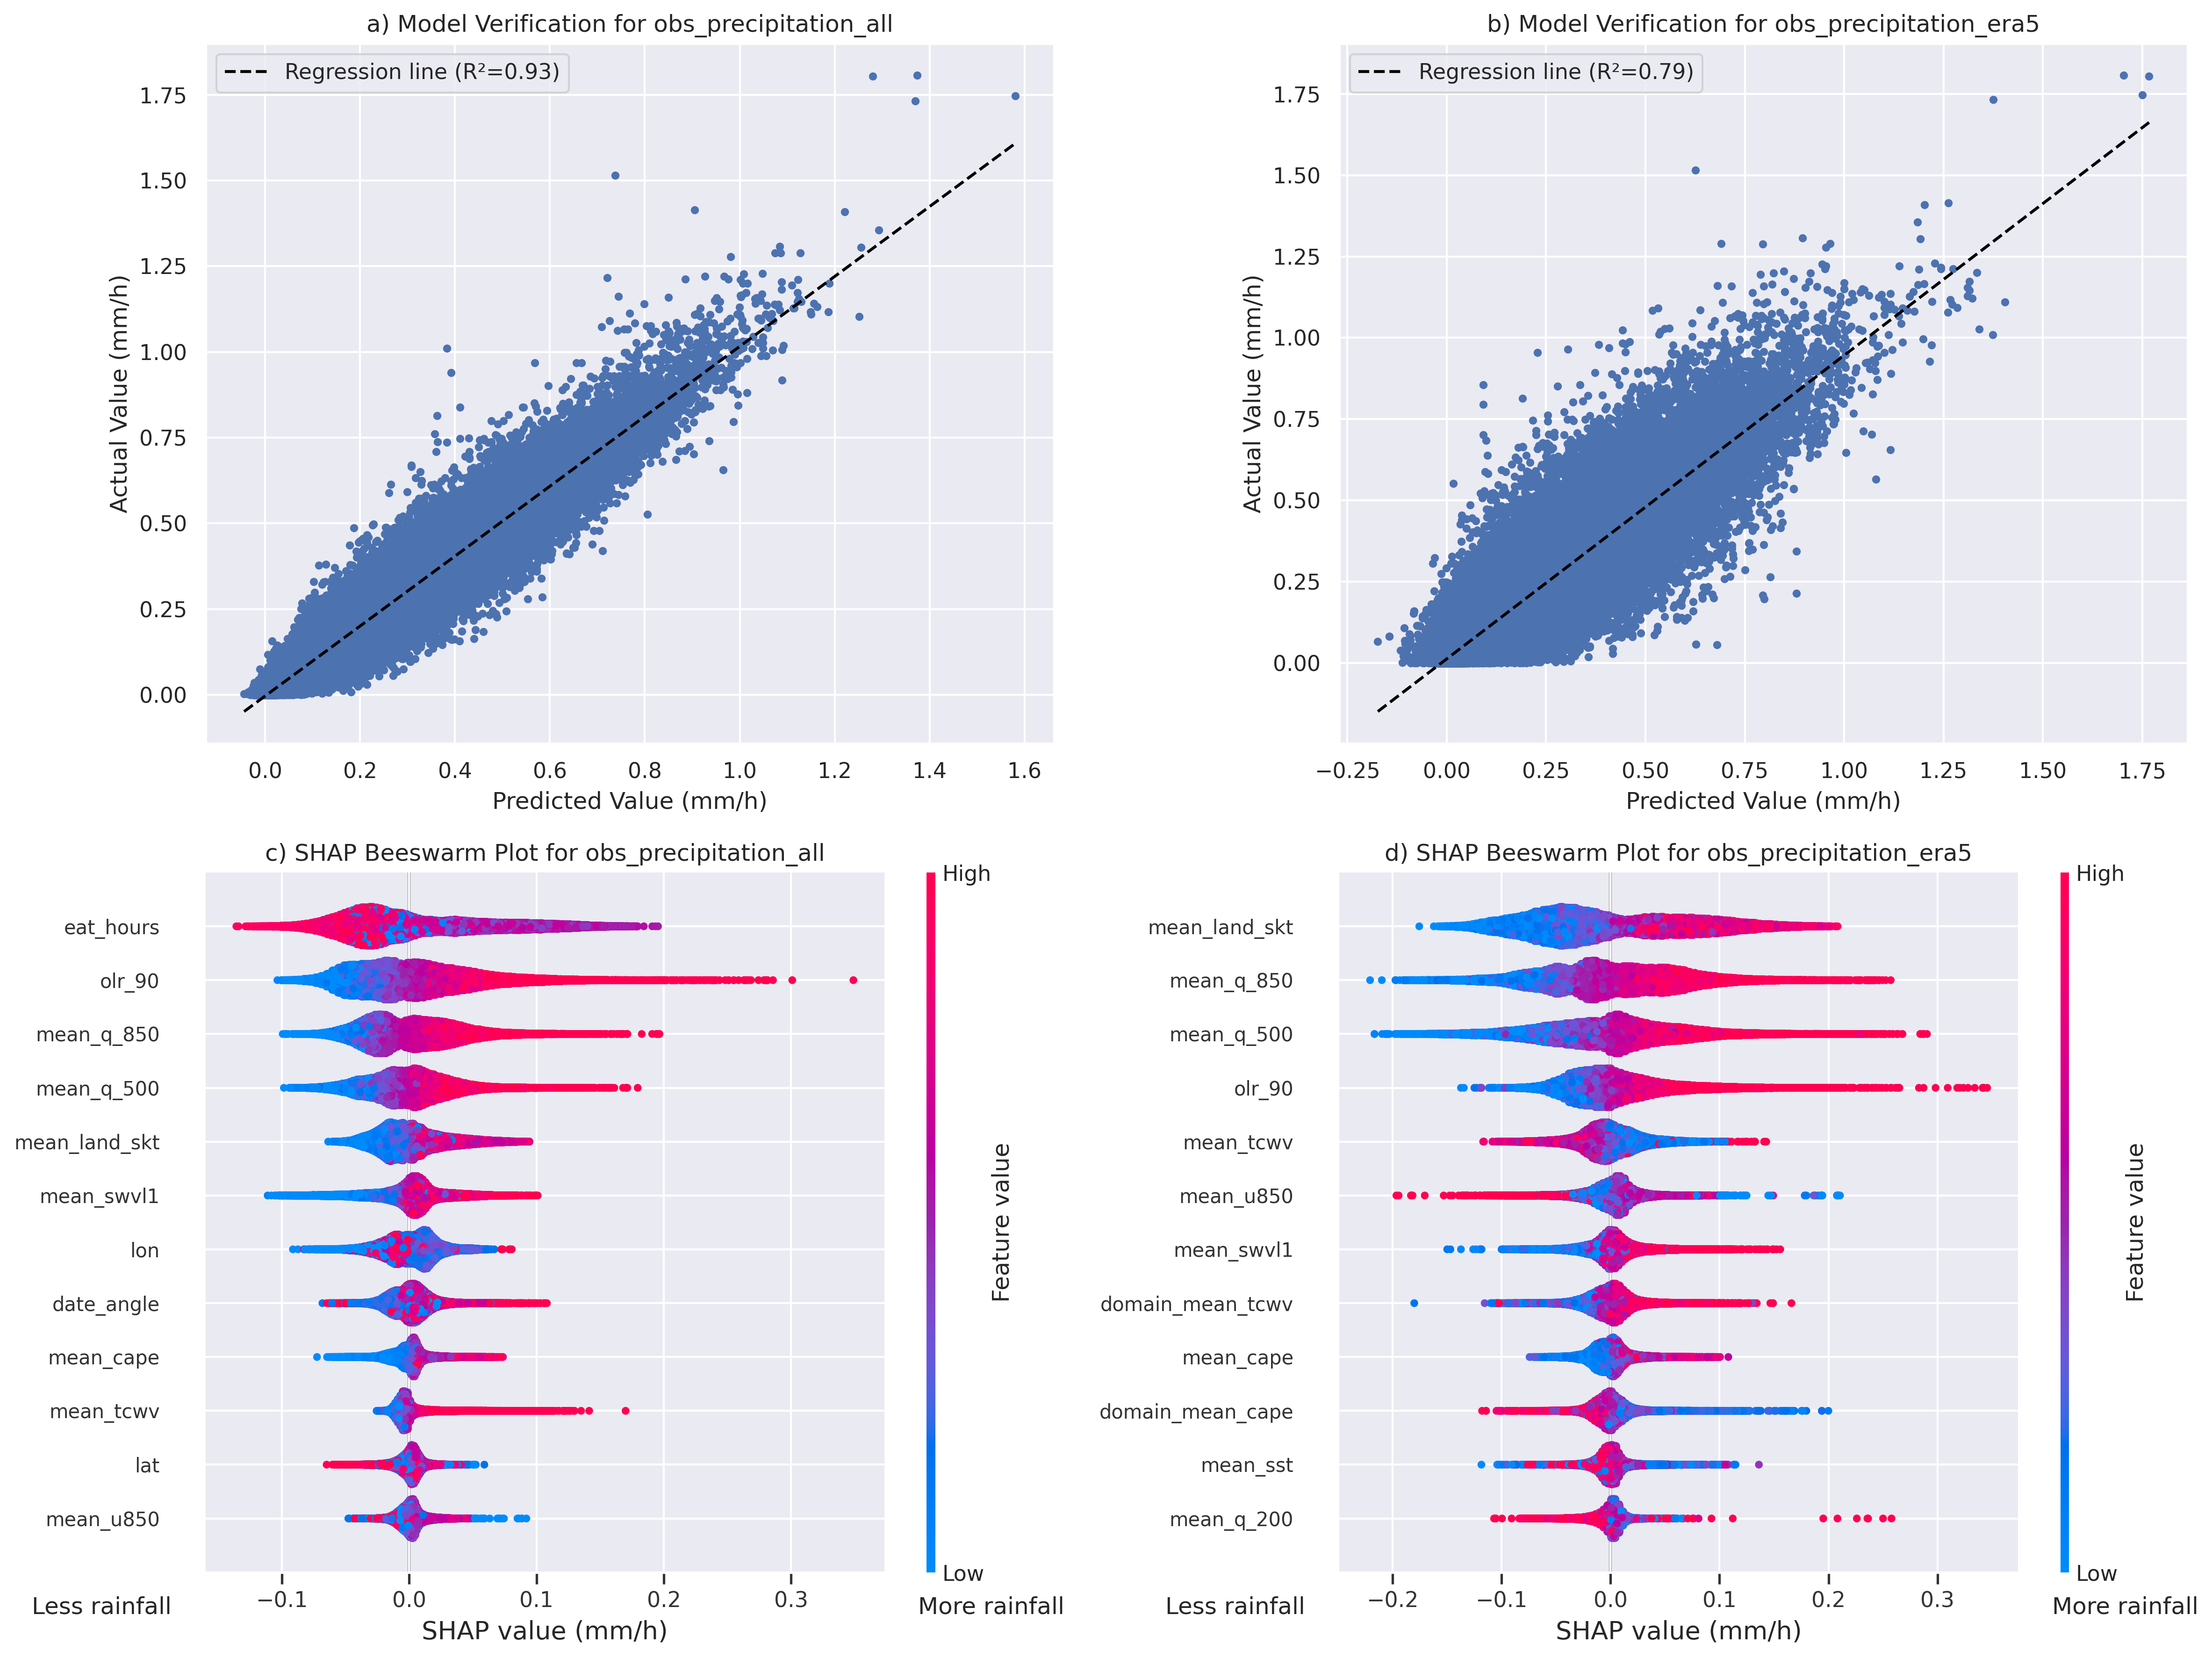
\includegraphics[width=\textwidth]{../figures/generated/experiments/obs_precipitation/obs_precipitation_summary.png}
    \caption{Comparison of performance and top features for precipitation.}
    \label{fig:obs_precipitation_summary}
\end{figure}

The \acrshort{era5} model appears to have captured the influence of the rainy seasons \todo{\acrshort{itcz}?} on precipitation patterns via the mean \acrshort{cape} over the study region as shown in Figure \ref{fig:obs_precipitation_era5_shap_domain_mean_cape_by_week_over_year}.

\begin{figure}[ht]
    \centering
    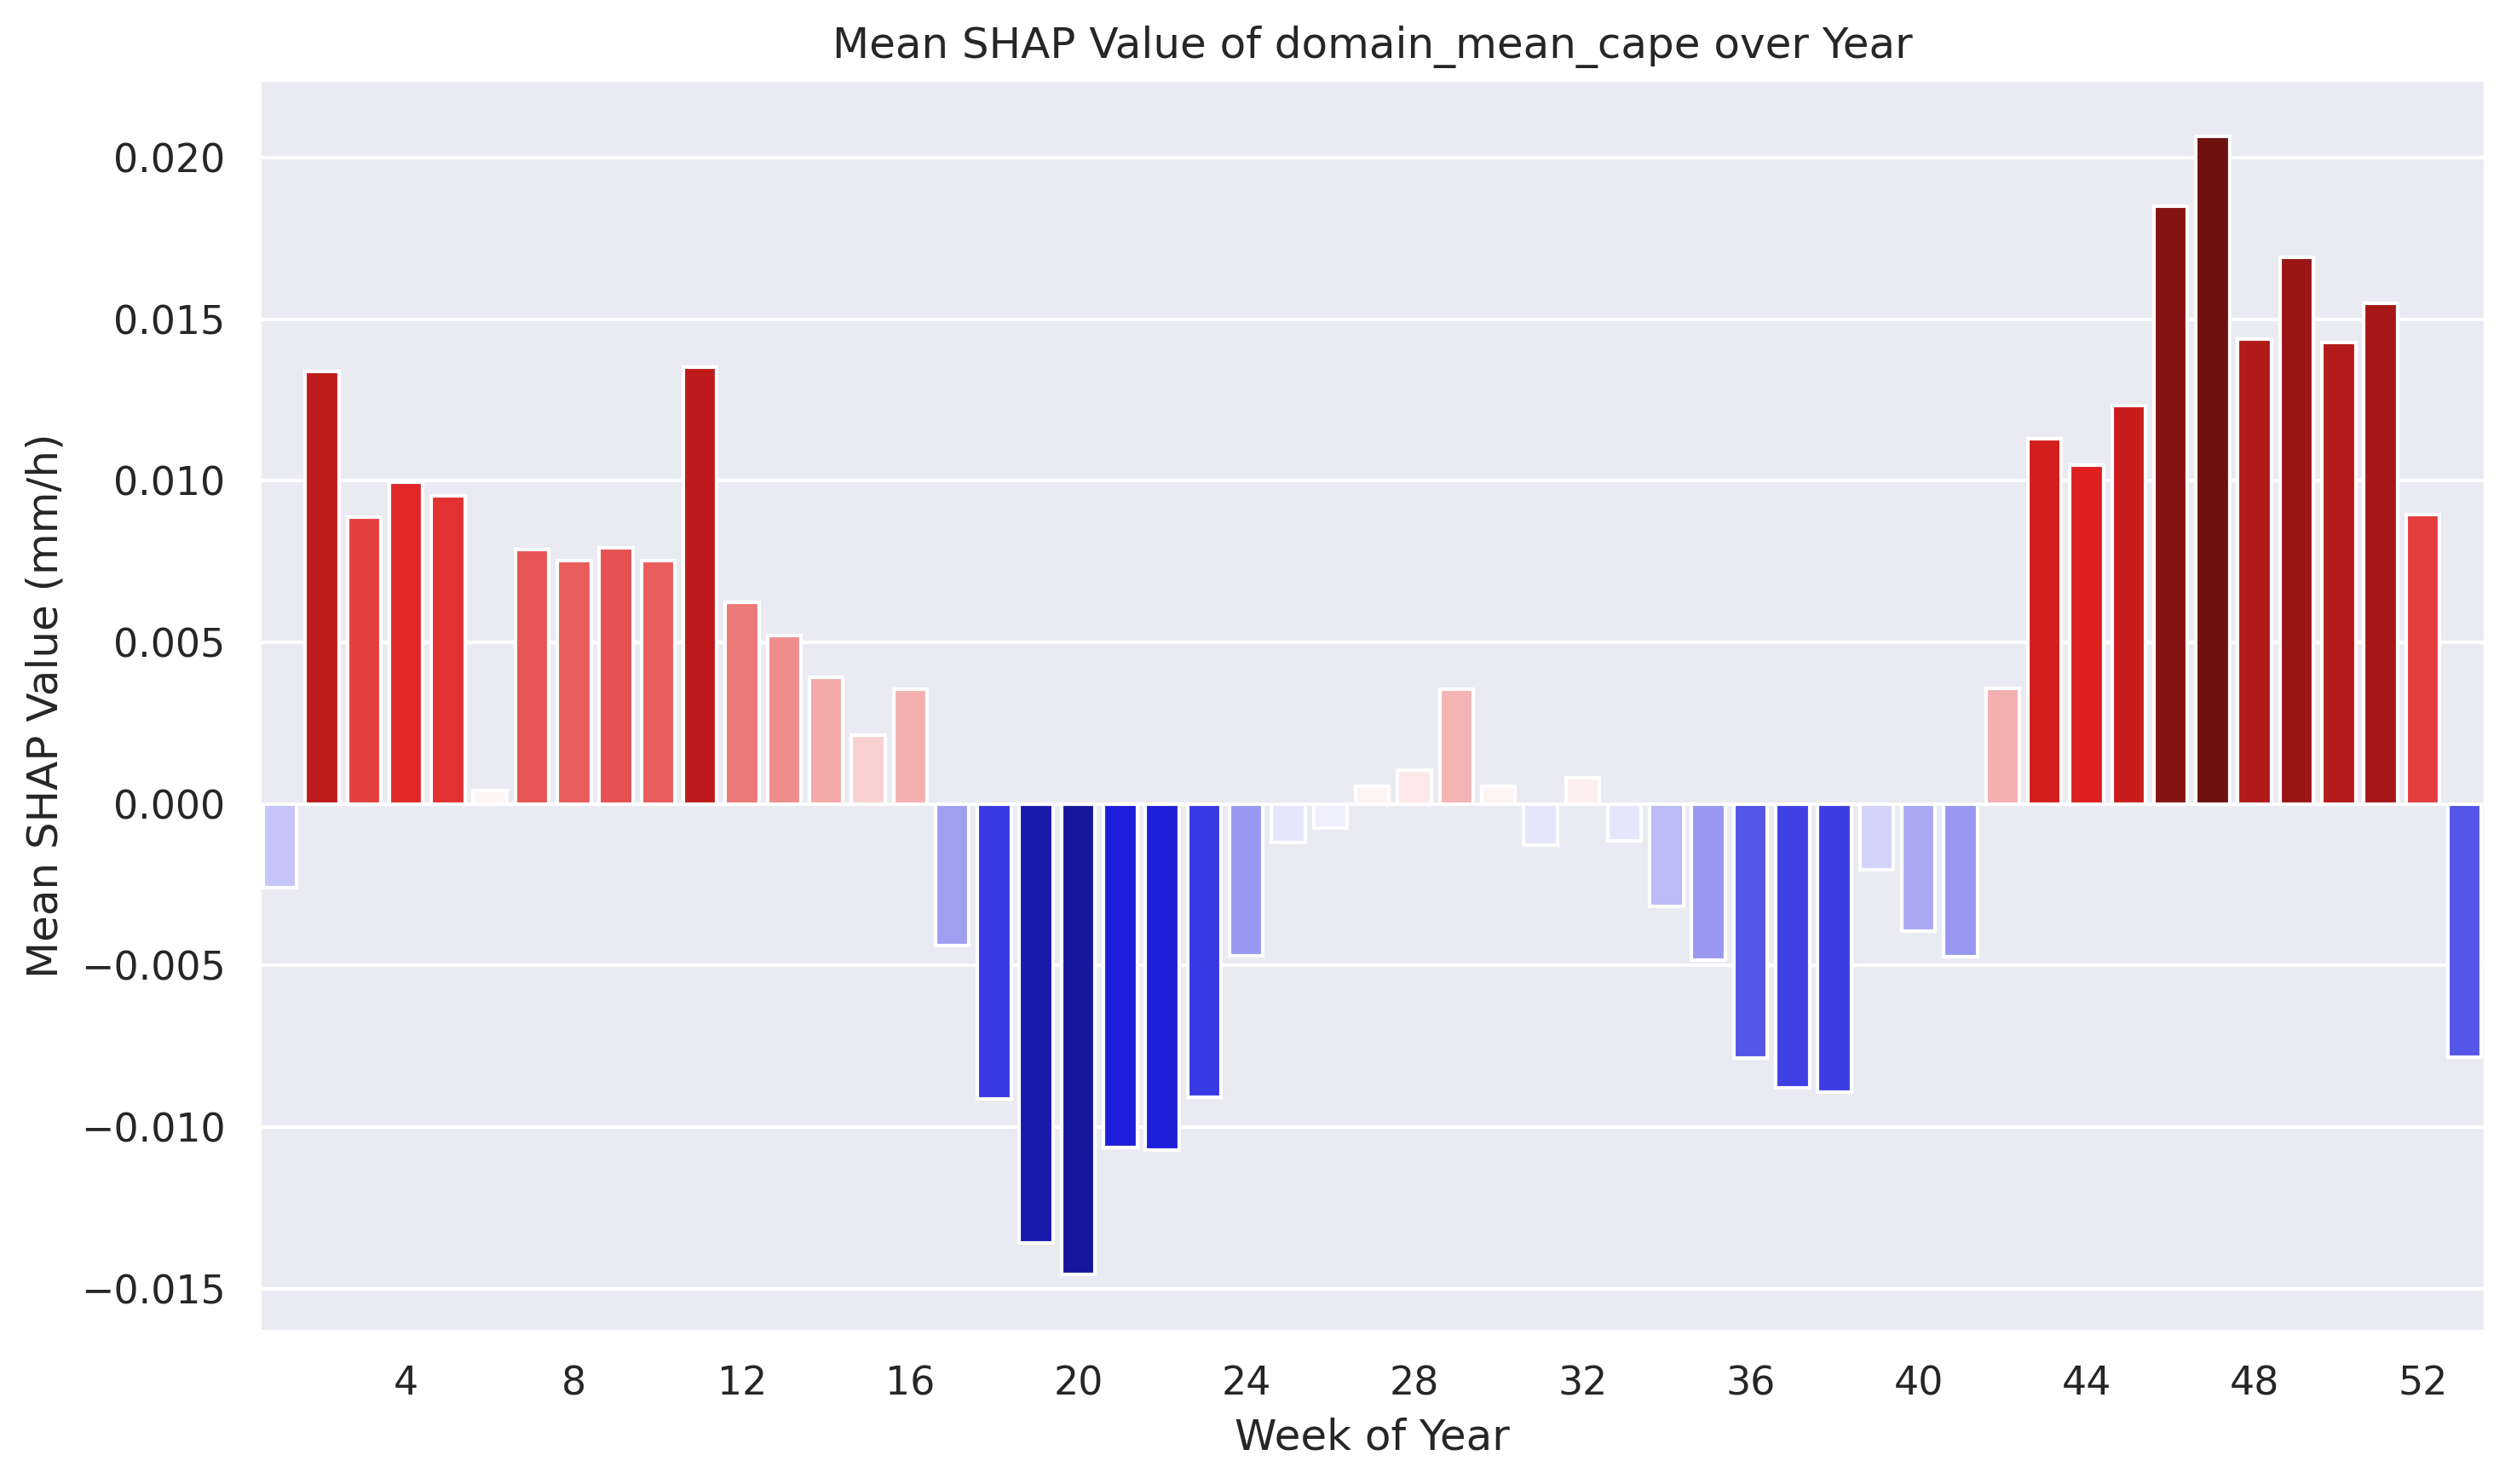
\includegraphics[width=\textwidth]{../figures/generated/experiments/obs_precipitation/temporal_corr/obs_precipitation_era5_shap_domain_mean_cape_by_week_over_year.png}
    \caption{Temporal variability of SHAP values for domain mean \acrshort{cape} by week over the year for the \acrshort{era5} model.}
    \label{fig:obs_precipitation_era5_shap_domain_mean_cape_by_week_over_year}
\end{figure}